\documentclass[a4paper, 8pt, landscape]{scrartcl}
\usepackage[german]{babel}
\usepackage[utf8]{inputenc}
\usepackage{multicol}
\usepackage{geometry}
\usepackage{graphicx}
\usepackage{wrapfig}
\usepackage{enumitem}
\usepackage{fancyhdr}
\usepackage{index}
\usepackage{sectsty}
\usepackage{mwe}
\usepackage{comment}
\usepackage{lipsum}
\usepackage{titlesec}
\usepackage[dvipsnames]{xcolor}
\usepackage{amsmath}
\usepackage{amssymb}
\usepackage{listings}

%Define Math Commands:
\newcommand*{\field}[1]{\mathbb{#1}}%
\newcommand{\Mod}[1]{\ (\mathrm{mod}\ #1)}

%Image Folder:
\graphicspath{{./img/}}

%format
\geometry{top=0.4cm,left=0.5cm,right=0.5cm,bottom=0.4cm}
\setlist{topsep=0pt, leftmargin=5mm, nolistsep}

% Code Snippets

\definecolor{javared}{rgb}{0.6,0,0} % for strings
\definecolor{javagreen}{rgb}{0.25,0.5,0.35} % comments
\definecolor{javapurple}{rgb}{0.5,0,0.35} 

\lstset{
language=Java,
basicstyle=\fontsize{8}{8} \ttfamily,
keywordstyle=\bfseries\color{javapurple},
stringstyle=\color{javared},
commentstyle=\color{javagreen},
morecomment=[s][\color{MidnightBlue}]{/**}{*/},
tabsize=2,
showspaces=false,
showstringspaces=false,
texcl = true,
rulecolor = \color{black},
breaklines = true,
aboveskip = 0.5em,
belowskip = 0em
}




% Define Section Format
\titleformat{name=\section}[block]
{\sffamily\normalsize}
{}
{0pt}
{\colorsection}
\titlespacing*{\section}{0pt}{3pt}{3pt}

\newcommand{\colorsection}[1]{%
\colorbox{MidnightBlue!40}{\parbox{0.98\linewidth}{\color{black}\thesection\ #1}}}


% Define Subsection Format
\titleformat{name=\subsection}[block]
{\sffamily\small}
{}
{0pt}
{\colorsubsection}
\titlespacing*{\subsection}{0pt}{3pt}{3pt}

\newcommand{\colorsubsection}[1]{%
\colorbox{YellowGreen!50}{\parbox{0.98\linewidth}{\color{black}\thesubsection\ #1}}}

% Define SubSubsection Format
\titleformat{name=\subsubsection}[block]
{\sffamily\small}
{}
{0pt}
{\colorsubsubsection}
\titlespacing*{\subsubsection}{0pt}{3pt}{3pt}

\newcommand{\colorsubsubsection}[1]{%
\colorbox{Goldenrod!50}{\parbox{0.98\linewidth}{\color{black}\thesubsubsection\ #1}}}

% -----------------------------------------------------------------------
\begin{document}
    %	\pagecolor{p}
    %	\color{t}
    \setlength{\columnseprule}{0.4pt}
    \footnotesize
    \begin{multicols*}{2}

        %! Author = Philipp Emmenegger
%! Date = 30/06/2021

\section{Einführung}
\textbf{Nutzen ComBau}
\begin{itemize}
    \item Programmiersprachen und Sprachkonzepte besser verstehen
    \item Sprachfeatures beurteilen können
    \item Konzepte in verwandten Bereichen einsetzen
\end{itemize}

\subsection{Begriffe}
\textbf{Compiler}
\begin{itemize}
    \item Transformiert Quellcode in Maschinencode
\end{itemize}
\textbf{Runtime System}
\begin{itemize}
    \item Unterstützt die Programmausführung mit Software und Hardware Mechanismen
\end{itemize}
\textbf{Syntax}
\begin{itemize}
    \item Definiert Struktur des Programms
    \item Bewährte Formalismen für Syntax
\end{itemize}
\textbf{Semantik}
\begin{itemize}
    \item Definiert Bedeutung des Programms
    \item Meist in Prosa beschrieben
\end{itemize}

\subsection{Architekturen}
\begin{center}
    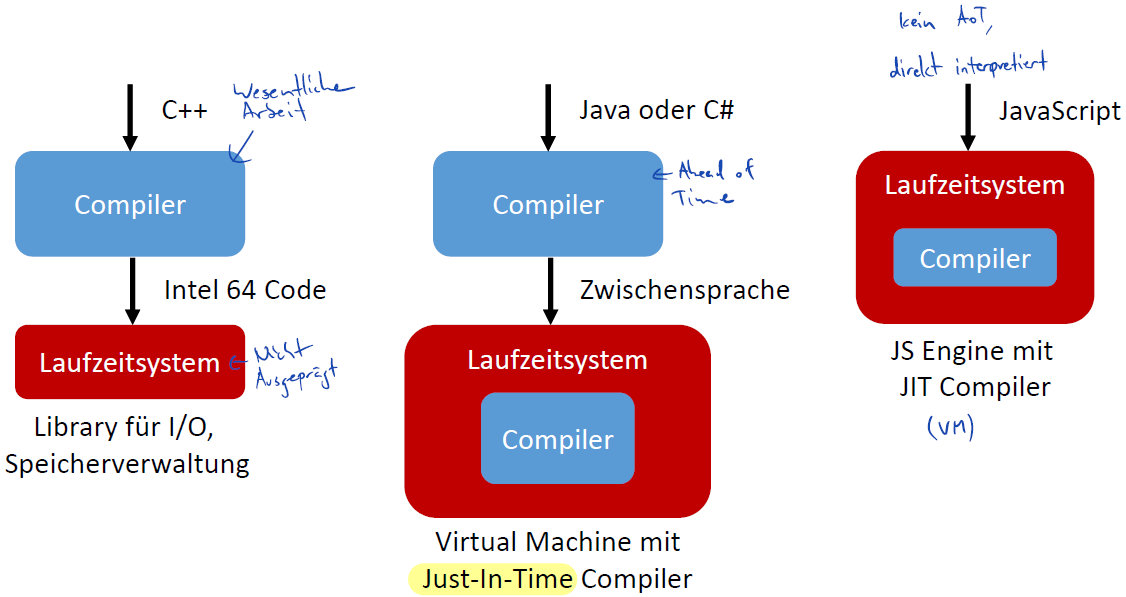
\includegraphics[width=0.6\linewidth]{/architekturen.png} 
\end{center}

\subsection{Aufbau Compiler}
\begin{center}
    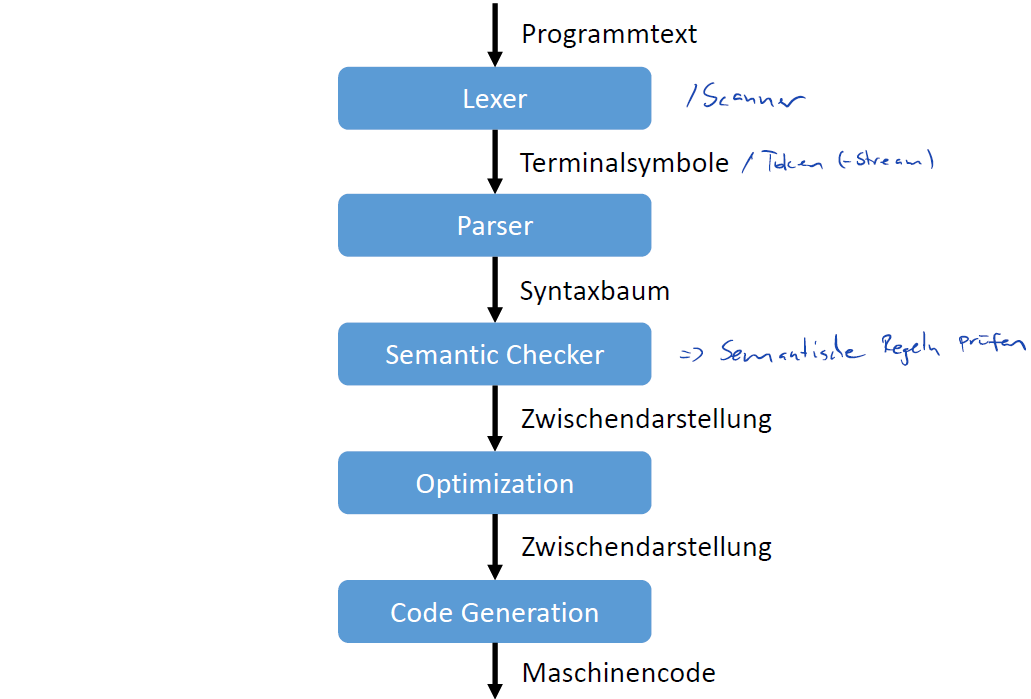
\includegraphics[width=0.5\linewidth]{/aufbau_compiler.png} 
\end{center}
\subsubsection{Lexer}
\textbf{Lexikalische Analyse, Scanner}
\begin{itemize}
    \item Zerlegt Programmtext in Terminalsymbole (Tokens)
    \item keine Tiefenstruktur
\end{itemize}
\subsubsection{Parser}
\textbf{Syntaktische Analyse}
\begin{itemize}
    \item Erzeugt Syntaxbaum gemäss Programmstruktur
    \item Kontextfreie Sprache
\end{itemize}
\subsubsection{Semantic Checker}
\textbf{Semantische Analyse}
\begin{itemize}
    \item Löst Symbole auf
    \item Prüft Typen und semantische Regeln
\end{itemize}
\subsubsection{Optimization}
\begin{itemize}
    \item Wandelt Zwischendarstellung in effizientere um
\end{itemize}
\subsubsection{Code Generation}
\begin{itemize}
    \item Erzeugt ausführbarer Maschinencode
\end{itemize}
\subsubsection{Zwischenarstellung}
\textbf{Intermediate Representation}
\begin{itemize}
    \item Beschreibt Programm als Datenstruktur (diverse Varianten)
\end{itemize}

\subsection{Aufbau Laufzeitsystem}
\begin{center}
    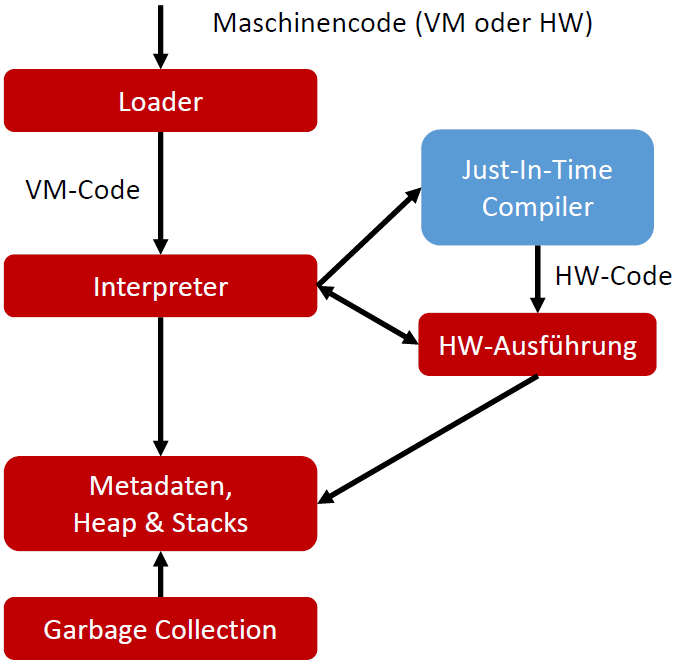
\includegraphics[width=0.4\linewidth]{/aufbau_laufzeitsystem.png} 
\end{center}
\subsubsection{Loader}
\begin{itemize}
    \item Lädt Maschinencode in Speicher
    \item Veranlasst Ausführung
\end{itemize}
\subsubsection{Interpreter}
\begin{itemize}
    \item Liest Instruktionen und emuliert diese in Software
\end{itemize}
\subsubsection{JIT (Just-In-Time) Compiler}
\begin{itemize}
    \item Übersetzt Code-Teile in Hardware-Instruktionscode
\end{itemize}
\subsubsection{HW-Ausführung (nativ)}
\begin{itemize}
    \item Lässt Instruktionscode direkt auf HW-Prozessor laufen
\end{itemize}
\subsubsection{Metadaten, Heap + Stacks}
\begin{itemize}
    \item Merken Programminfos, Objekte und Prozeduraufrufe
\end{itemize}
\subsubsection{Garbage Collection}
\begin{itemize}
    \item Räumt nicht erreichbare Objecte ab
\end{itemize}
\newpage

\subsection{Syntax}
\subsubsection{EBNF}
\textbf{Extended Backus-Naur Form}
\begin{center}
    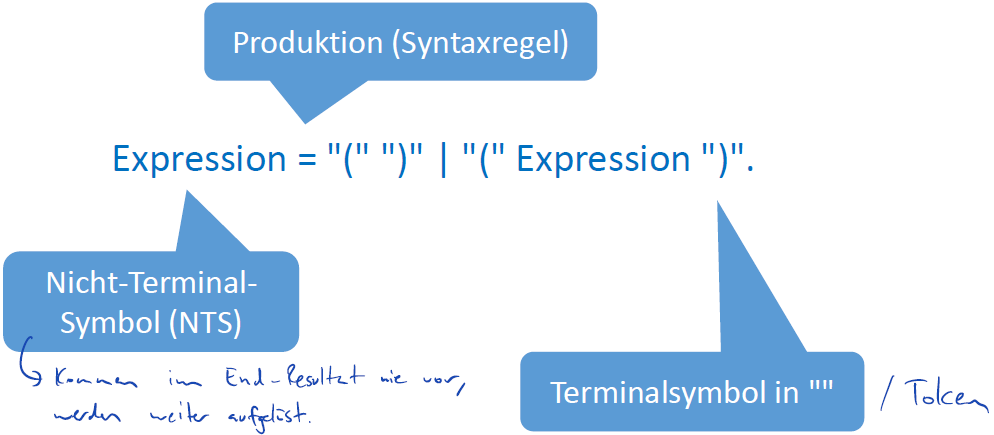
\includegraphics[width=0.5\linewidth]{/ebnf.png} 
    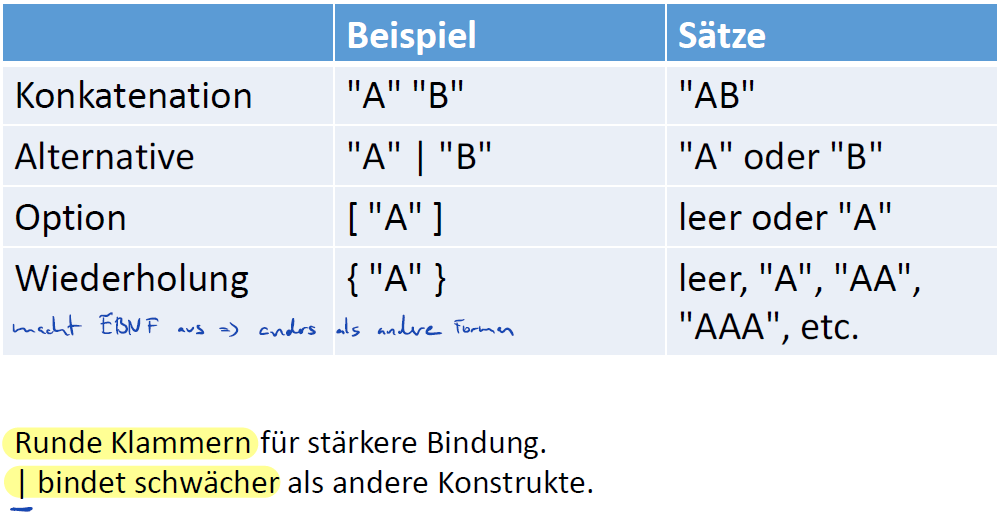
\includegraphics[width=0.5\linewidth]{/ebnf_regeln.png} 
\end{center}
\subsubsection{Arithmetische Ausdrücke}
\begin{center}
    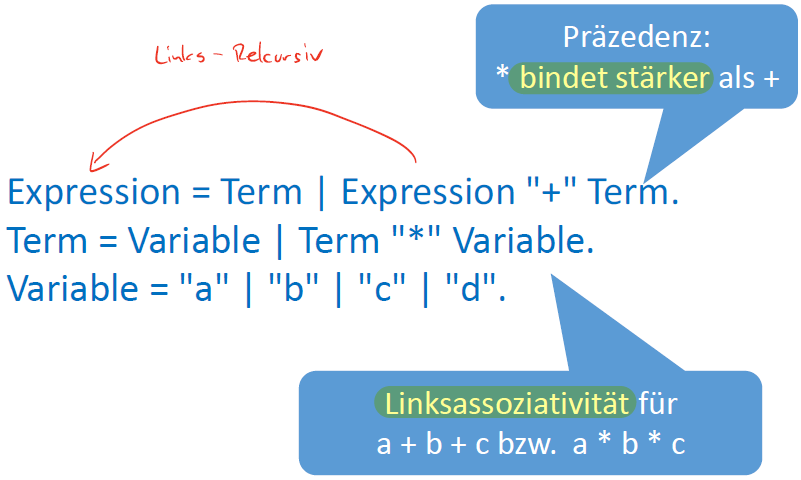
\includegraphics[width=0.5\linewidth]{/ebnf_arithmetisch.png} 
\end{center}
        \newpage
        \section{Lexikalische Analyse}
\subsection{Lexer / Scanner}
\textbf{Endlicher Automat (DEA)}
\begin{itemize}
    \item Kümmert sich um die lexikalische Analyse
    \item Input: Zeichenfolge (Programmtext)
    \item Output: Folge von Terminalsymbolen (Tokens)
\end{itemize}
\subsubsection{Aufgaben}
\begin{itemize}
    \item Fasst Textzeichen zu tokens zusammen
    \item Eliminiert Whitespaces
    \item Eliminiert Kommentare
    \item Merkt Positionen in Programmcode
\end{itemize}
\subsubsection{Nutzen}
\textbf{Abstraktion}
\begin{itemize}
    \item Parser muss sich nicht um Textzeichen kümmern
\end{itemize}
\textbf{Einfachheit}
\begin{itemize}
    \item Parser braucht Lookahead pro Symbol, nicht Textzeichen
\end{itemize}
\textbf{Effizienz}
\begin{itemize}
    \item Lexer benötigt keinen Stack im Gegensatz zu Parser
\end{itemize}

\subsection{Tokens}
\textbf{Statisch (Keywords, Operationen, Interpunktion)}
\begin{itemize}
    \item \textit{if}
    \item \textit{else}
    \item \textit{while}
    \item \textit{*}
    \item \textit{\&\&}
    \item \textit{;}
\end{itemize}
\textbf{Identifiers}
\begin{itemize}
    \item MyClass
    \item readFile
    \item name2
\end{itemize}
\textbf{Zahlen}
\begin{itemize}
    \item 123
    \item 0xfe12
    \item 1.2e-3
\end{itemize}
\textbf{Strings}
\begin{itemize}
    \item \dq Hello\dq
    \item \dq \dq
    \item \dq $\backslash$n\dq
\end{itemize}
\begin{center}
    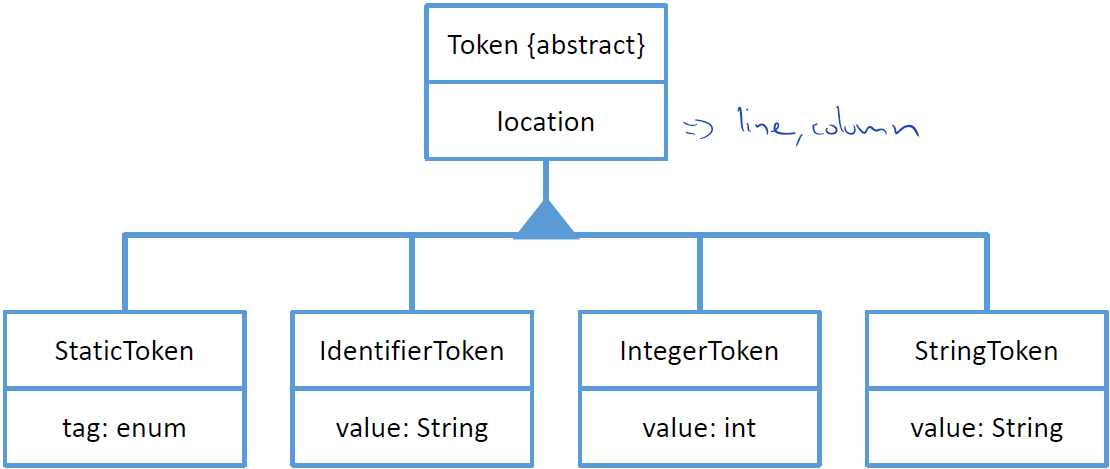
\includegraphics[width=0.4\linewidth]{/token_model.png} 
\end{center}

\subsubsection{Lexem}
\begin{itemize}
    \item Spezifische Zeichenfolge, die einen Token darstellt
    \item z.B. \textit{MyClass} ist ein Lexem des Tokens Identifier
\end{itemize}

\subsubsection{Maximum Munch}
\begin{itemize}
    \item Lexer absorbiert möglichst viel in einem Token
\end{itemize}

\subsection{Reguläre Sprachen}
\begin{itemize}
    \item Lexer unterstützt nur reguläre Sprachen
    \item \textbf{Regulär:} Als EBNF ohne Rekursion ausdrückbar
\end{itemize}
\begin{center}
    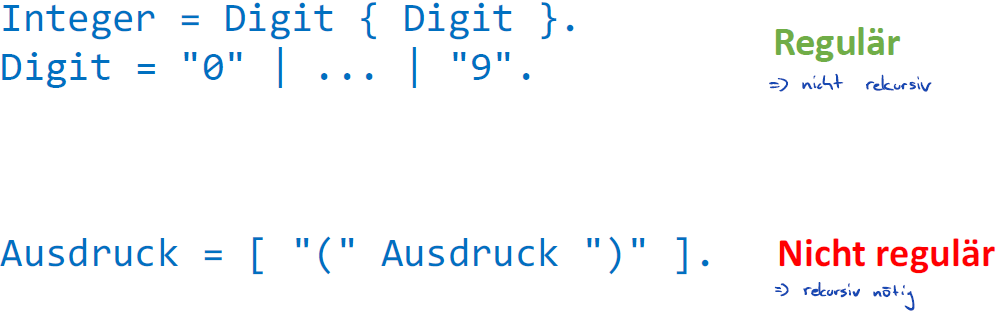
\includegraphics[width=0.5\linewidth]{/reg_sprachen.png} 
\end{center}

\subsection{Chomsky Hierarchie}
\begin{center}
    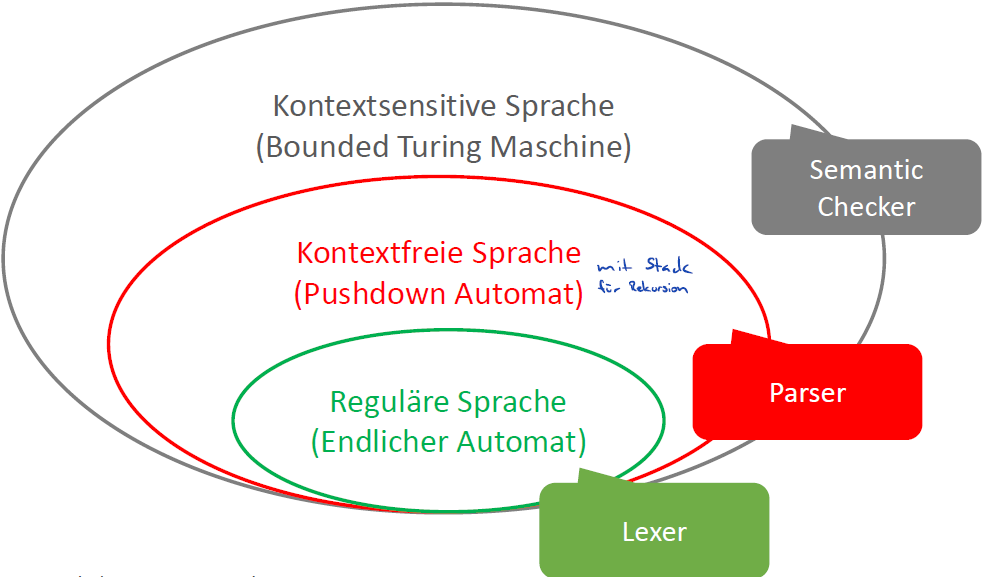
\includegraphics[width=0.7\linewidth]{/chomsky.png} 
\end{center}

\subsection{Lexer Gerüst}
\begin{lstlisting}
class Lexer {
    private final Reader reader;
    private char current; // one Character Lookahead
    private boolean end; // EOF 

    private Lexer(Reader reader) {
        this.reader = reader;
    }

    public static Iterable<Token> scan(Reader reader) {
        return new Lexer(reader).readTokenStream();
    }

    // ...
}
\end{lstlisting}

\subsection{Token Stream lesen}
\begin{lstlisting}
Iterable<Token> readTokenStream() {
    var stream = new ArrayList<Token>();
    readNext(); // One Character Lookahead
    skipBlanks();
    while (!end) {
        stream.add(readToken());
        skipBlanks();
    }
    return stream;
}
\end{lstlisting}

\subsection{Lexer Kernlogik}
\begin{lstlisting}
Token readToken() {
    if(isDigit(current)) {
        return readInteger();
    }
    if(isLetter(current)) {
        return readName(); // Identifier / Keyword 
    }
    return switch(current) {
        case '"': readString();
        case '+': readStaticToken(Tag.Plus);
        case '-': readStaticToken(Tag.Minus);
        case '/': readPotentialSlash();
    }
}
\end{lstlisting}

\subsubsection{Static Token scannen}
\begin{lstlisting}
StaticToken readStaticToken(Tag tag) {
    readNext();
    return new StaticToken(tag);
}
\end{lstlisting}

\subsubsection{Zahlen scennen}
\textbf{Beachten:}
\begin{itemize}
    \item Range Check (32 bit): Integer Overflow
    \item $Integer.MIN$ = $Integer.MAX+1$
\end{itemize}
\begin{lstlisting}
IntegerToken readInteger() {
    int value = 0;
    while (!_end && isDigit(current)) {
        int digit = current - '0'; // char to int 
        value = value * 10 + digit; // create decimal number
        readNext();
    }
    return new IntegerToken(value);
}
\end{lstlisting}

\subsubsection{Identifier und Keywords scannen}
\begin{lstlisting}
Token readName() {
    String name = Character.toString(current);
    readNext();
    while(!end & (isLetter(current) || isDigit(current))) {
        name += current;
        readNext();
    }
    if(KEYWORDS.containsKey(name)) {
        return new StaticToken(KEYWORDS.get(name));
    }
    return new IdentifierToken(name);
}
\end{lstlisting}

\subsubsection{String scannen}
\textbf{Beachten:}
\begin{itemize}
    \item Kein $\backslash$t
    \item Kein $\backslash$\dq
    \item Kein $\backslash$n
    \item Keine mehrzeiligen Strings
\end{itemize}
\begin{lstlisting}
StringToken readString() {
    readNext(); // Skip leading double Quote
    String value = "";
    while (!end && current != '"') {
        value += current;
        readNext();
    }
    if(end) {
        // Error: String not closed
    }
    readNext(); // Skip trailing double Quote
    return new StringToken(value);
}
\end{lstlisting}

\subsubsection{Kommentare erkennen}
\begin{lstlisting}
StaticToken readPotentialSlash() {
    readNext();
    if(current == '/') {
        skipLineComment();
        // move on to next token
    } else if (current == '*') {
        skipCommentBlock();
        // move on to next token
    } else {
        return new StaticToken(Tag.Divide);
    }
}
\end{lstlisting}
        \newpage
        \section{Parser}
\textbf{Kontextfreie Sprache}
\begin{itemize}
    \item Kümmert sich um die syntaktische Analyse
    \item Input: Tokens (Terminalsymbole)
    \item Output: Syntaxbaum / Parse Tree
\end{itemize}
\subsection{Aufgabe}
\begin{itemize}
    \item Finde eindeutige Ableitung der Syntaxregeln, um einen gegebenen Input herzuleiten
    \item Analysiert die gesamte Syntaxdefinition (mit rekursiven Regeln)
    \item Erkennt, ob Eingabetext Syntax erfüllt
    \item Erzeugt Syntaxbaum
\end{itemize}
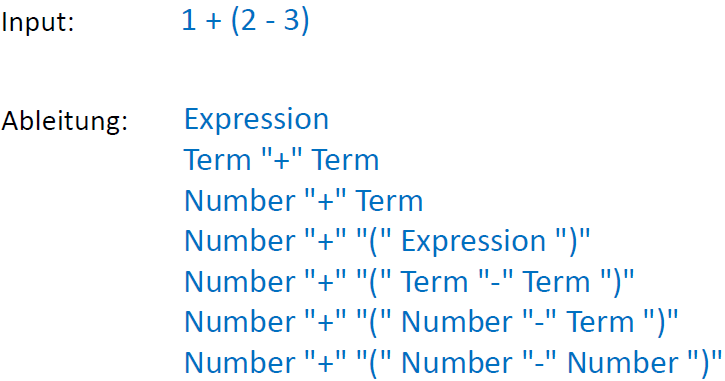
\includegraphics[width=0.5\linewidth]{/parser_aufgabe.png} 

\subsection{Parse Tree}
\begin{itemize}
    \item Concrete Syntax Tree
    \item Ableitung der Syntaxregeln als Baum wiedergespiegelt
    \item Kann generiert werden
\end{itemize}
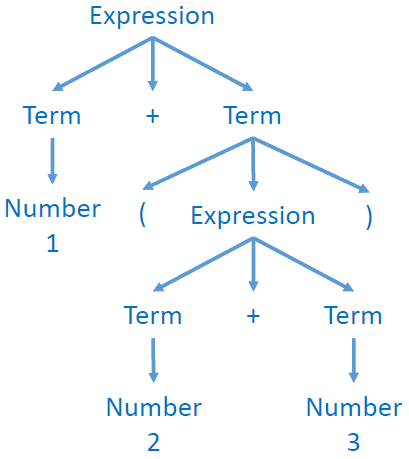
\includegraphics[width=0.3\linewidth]{/parse_tree.png} 

\subsubsection{Abstract Syntax Tree}
\begin{itemize}
    \item Unwichtige Details auslassen
    \item Struktur vereinfacht
    \item Für Weiterverarbeitung massgeschneidert
    \item Eigendesign nach Gusto des Compiler-Entwicklers
    \item Nur mit Selbstimplementation möglich
\end{itemize}
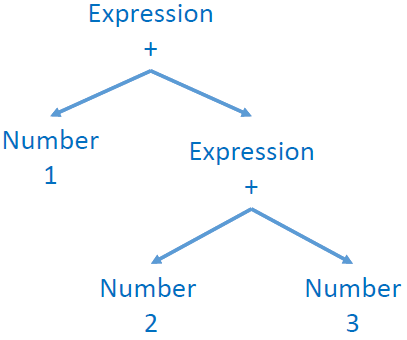
\includegraphics[width=0.3\linewidth]{/abstract_parse_tree.png} 

\subsection{Parser Strategien}
\subsubsection{Top-Down}
\begin{itemize}
    \item Beginne mit Start-Symbol
    \item Wende Produktionen an
    \item Expandiere Start-Symbol auf Eingabetext
    \item $Expr -> Term + Term -> ... -> 1 + (2 - 3)$
\end{itemize}
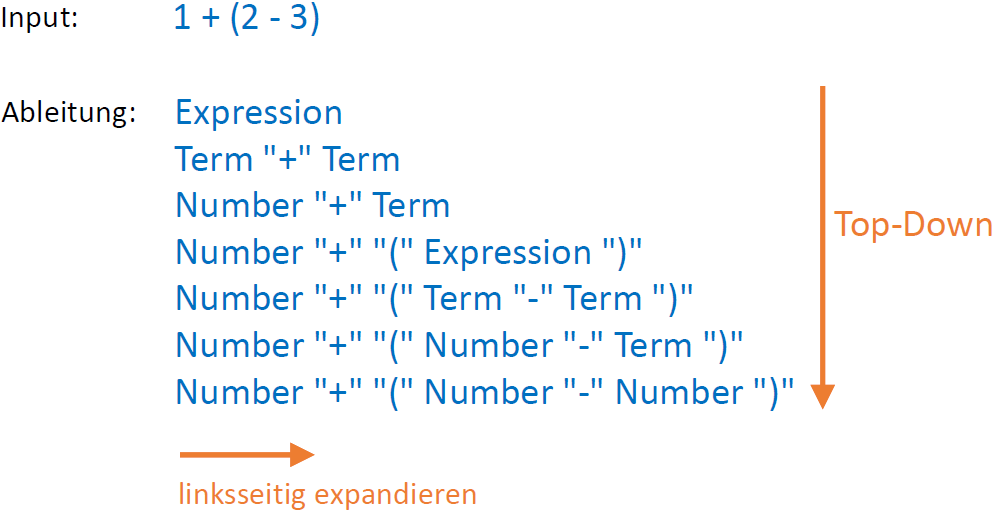
\includegraphics[width=0.5\linewidth]{/top_down.png} 

\subsubsection{Bottom-Up}
\begin{itemize}
    \item Beginne mit Eingabetext
    \item Wende Produktionen an
    \item Reduziere Eingabetext auf Start-Symbol
    \item $Expr <- Term + Term <- ... <- 1 + (2 - 3)$
\end{itemize}
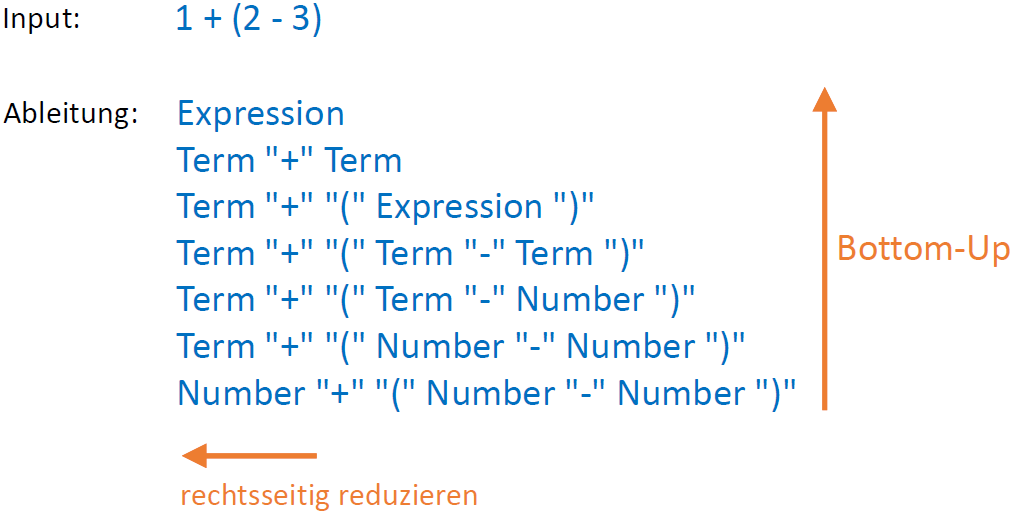
\includegraphics[width=0.5\linewidth]{/bottom_up.png} 

\subsection{Recursive Descent}
\begin{itemize}
    \item Pro Nicht-Terminalsymbol eine Methode
    \begin{itemize}
        \item Implementiert die Erkennung gemäss EBNF-Produktion
    \end{itemize}
    \item Vorkommen eines Nicht-Terminalsymbols in Syntax
    \begin{itemize}
        \item Aufruf der entsprechenden Methode
    \end{itemize}
    \item Funktioniert bei rekursiven und nicht-rekursiven Produktionen
\end{itemize}
\begin{lstlisting}
void parseExpression() {
    parseTerm();
    // ...
}
void parseTerm() {
    parseExpression();
    // ...
}
\end{lstlisting}

\subsection{Parser Gerüst}
\begin{lstlisting}
public class Parser {
    private final Iterator<Token> tokenStream;
    private Token current; // One Token Lookahead

    private Parser(Iterable<Token> tokenStream) {
        this.tokenStream = tokenStream.iterator();
    }

    public static ProgramNode parse(Iterable<Token> stream) {
        return new Parser(stream).parseProgram(); // Aufbasierte Klasse
    }
}
\end{lstlisting}

\subsubsection{Parser-Einstieg}
$Program = Expression$
\begin{lstlisting}
private ProgramNode parseProgram() {
    var classes = new ArrayList<ClassNode>();
    parseExpression();
    while (!isEnd()) {
        next();
        classes.add(parseClass());
    }
    return new ProgramNode(classes);
}
\end{lstlisting}

\subsubsection{Expression}
$Expression = Term { ( \dq +\dq | \dq -\dq ) Term }$
\begin{lstlisting}
Expression parseExpression() {
    var left = parseTerm();
    while(is(Tag.PLUS) || is(Tag.MINUS)) {
        var op = is(Tag.PLUS) ? Operator.PLUS : Operator.MINUS;
        next();
        var right = parseTerm();
        var left = new BinaryExpression(op, left, right);
    }
    return left;
}
\end{lstlisting}

\subsubsection{Term}
$Term = Number | \dq (\dq Expression \dq )\dq$
\begin{lstlisting}
Expression parseTerm() {
    if(isInteger()) {
        int value = readInteger();
        next();
        return new IntegerLiteral(value);
    } else if (is(Tag.OPEN_PARENTHESIS)) {
        next();
        var expression = parseExpression();
        if(is(Tag.CLOSE_PARENTHESIS)) {
            next();
        } else {
            error(); // missing closed parenthesis
        }
        return expression();
    } else {
        error(); // missing open parenthesis
    }
}
\end{lstlisting}

\subsection{One Symbol Lookahead}
\textbf{Statement}\\
$Assignment | IfStatement$
\begin{itemize}
    \item Bestimme mögliche Terminalsymbole, die mit einer Produktion ableitbar sind (FIRST-Menge)
    \item Benutze FIRST zur Entscheidung der Alternative beim zielorientierten Parsen
\end{itemize}
\begin{lstlisting}
void parseStatement() {
    if(isIdentifier()) { // FIRST(Assignment)
        parseAssignment();
    } else if(is(Tag.IF)) { // FIRST(IfStatement)
        parseIfStatement();
    } else {
        error();
    }
}
\end{lstlisting}

\subsection{Technische Syntax-Umformung}
\begin{itemize}
    \item Falls 1 Lookahead nicht reicht
\end{itemize}
\begin{lstlisting}
Statement = Assignment | Invocation
Assignment = Identifier "=" Expression
Invocation = Identifier "(" ")"
\end{lstlisting}

\begin{center}
    $\downarrow$
\end{center}

\begin{lstlisting}
Statement = Identifier (AssignmentRest | InvocationRest)
AssignmentRest = "=" Expression 
InvocationRest = "(" ")"
// Lookahead 1 reicht wieder
\end{lstlisting}

\subsubsection{Code Beispiel}
\begin{lstlisting}
var parseStatement() {
    var identifier = readIdentifier();
    next();
    if (is(Tag.ASSIGN)) {
        parseAssignmentRest(identifier);
    } else if (is(Tag.OPEN_PARENTHESIS)) {
        parseInvocationRest(identifier);
    } else {
        error();
    }
}
\end{lstlisting}
        \newpage
        \section{Parser Vertiefung}
\subsection{Abstrakter Syntaxbaum Design}
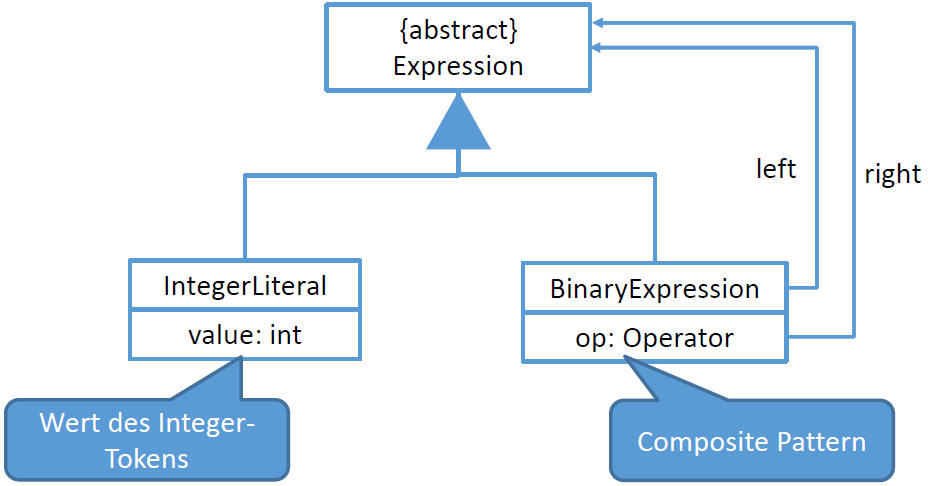
\includegraphics[width=0.7\linewidth]{syntaxbaum_design.png}

\subsection{Bottom-Up Parsing}
\begin{itemize}
    \item Mächtiger als LL (Top-Down) Parser
    \item Kann Linksrekursion behandeln
\end{itemize}
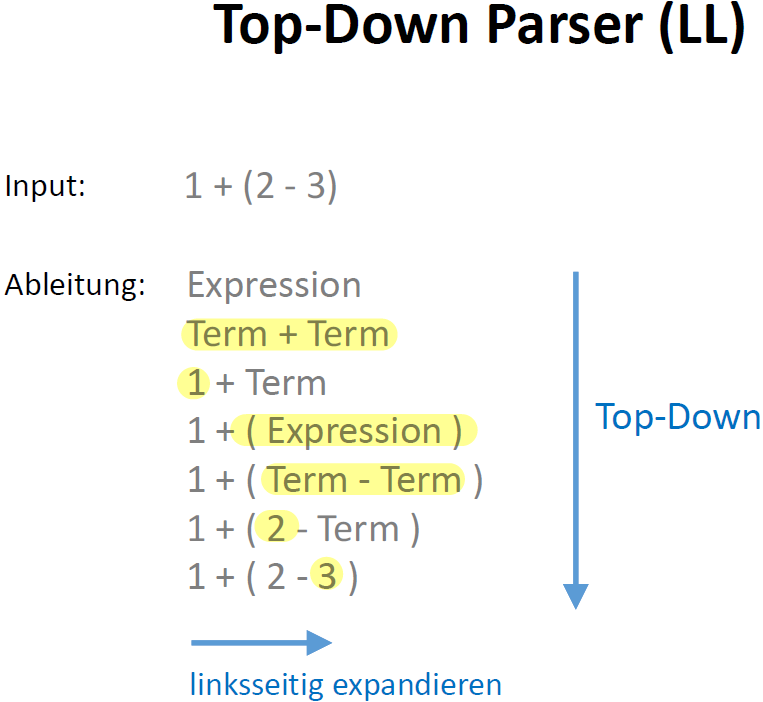
\includegraphics[width=0.5\linewidth]{top_down2.png}
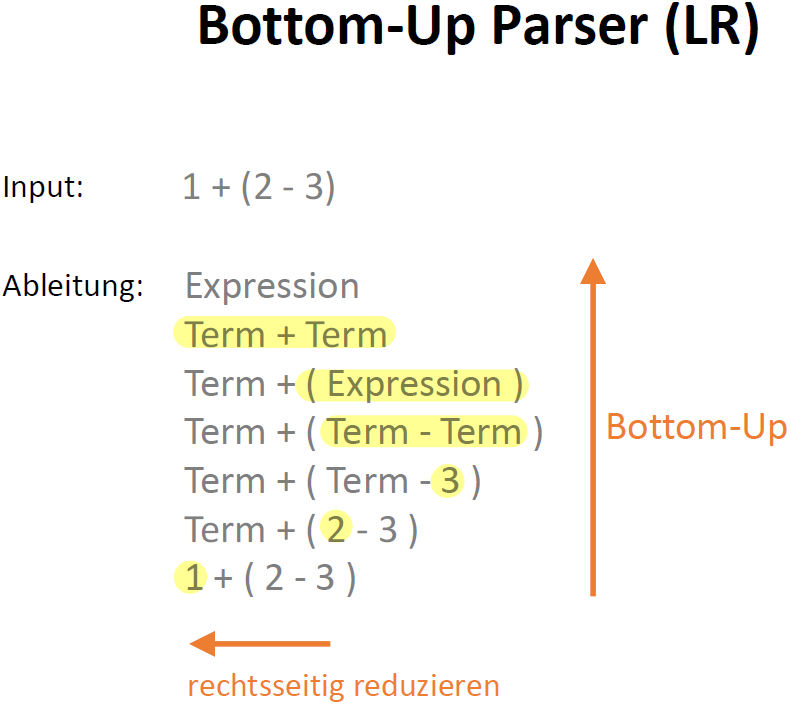
\includegraphics[width=0.5\linewidth]{bottom_up2.png}

\subsubsection{Ansatz}
\begin{itemize}
    \item Lese Symbole im Text ohne fixes Ziel
    \item Prüfe nach jedem Schritt, ob gelesene Folge Produktion entspricht
    \begin{itemize}
        \item Wenn ja: Reduziere auf Syntaxkonstrukt (REDUCE)
        \item Wenn nein: Lese weiteres Symbol im Text (SHIFT)
    \end{itemize}
    \item Am Schluss bleibt Startsymbol übrig, sonst Syntaxfehler
\end{itemize}

\subsubsection{Beispielablauf}
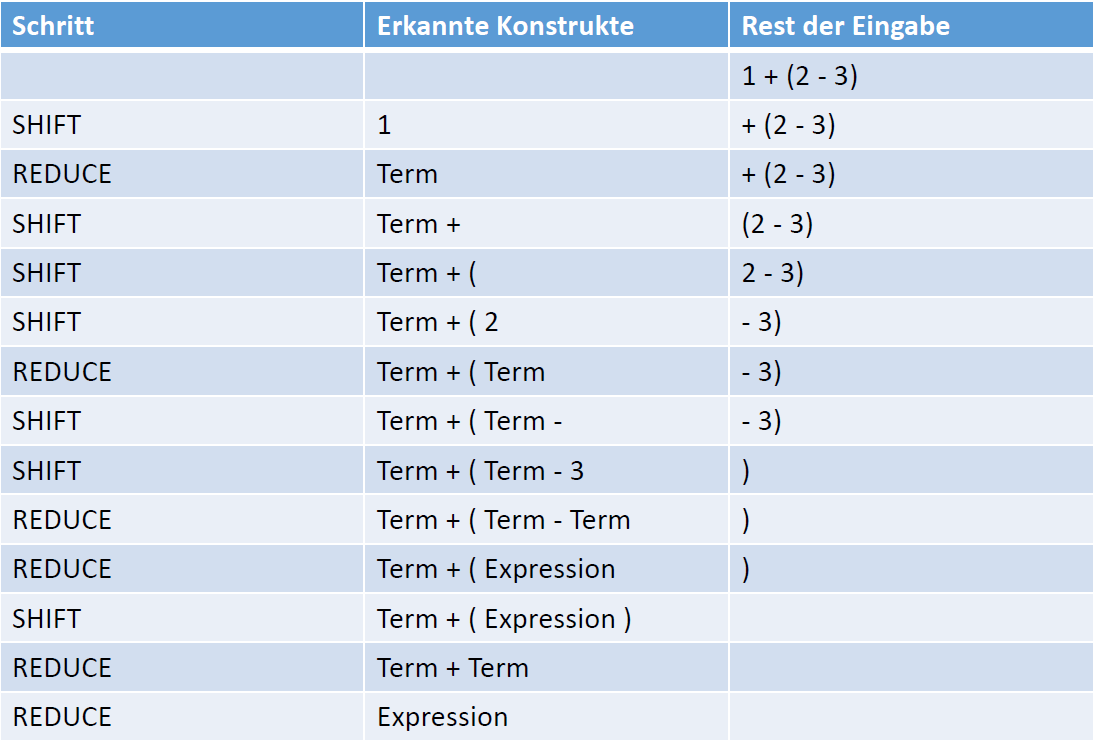
\includegraphics[width=0.7\linewidth]{bottom_up_ablauf.png}
\subsubsection{Parser Tabelle - Vereinfacht}
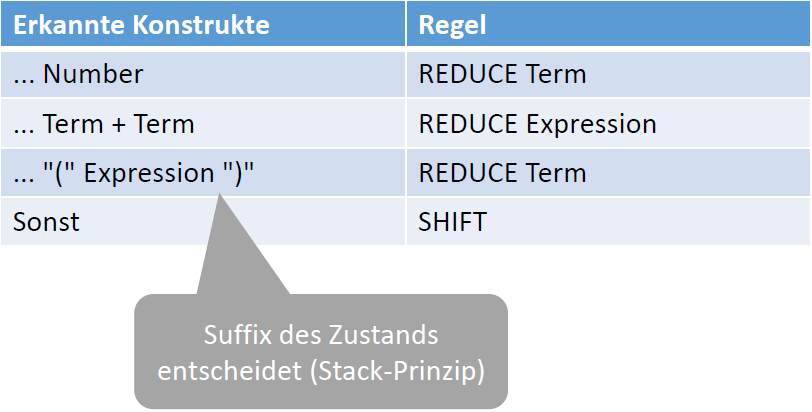
\includegraphics[width=0.5\linewidth]{parser_tabelle_vereinfacht.png}

\subsection{LR-Parser (Bottom-Up) Varianten}
\textbf{LR(0)}
\begin{itemize}
    \item Parse Tabelle ohne Lookahead erstellen
    \item Zustand reicht, um zu entscheiden
\end{itemize}
\textbf{SLR(k) (Simple LR)}
\begin{itemize}
    \item Lookahead bei REDUCE, um Konflikt zu lösen
    \item Keine neuen Zustände
\end{itemize}
\textbf{LALR(k) (Look-Ahead LR)}
\begin{itemize}
    \item Analysiert Sprache auf LR(0)-Konflikte
    \item Benutzt Lookahead bei Konfliktstellen mit neuen Zuständen
\end{itemize}
\textbf{LR(k)}
\begin{itemize}
    \item Pro Grammatikschritt + Lookahead ein Zustand
    \item Nicht praxistauglich, zu viele Zustände
\end{itemize}
        \newpage
        \section{Semantic Checker}
\begin{itemize}
    \item Kümmert sich um die semantische Analyse
    \item Input: Syntaxbaum
    \item Output: Zwischendarstellung (Syntaxbaum + Symboltabelle)
\end{itemize}
\subsection{Semantische Prüfung}
\textbf{Deklarationen}
\begin{itemize}
    \item Jeder Identifier ist eindeutig deklariert
\end{itemize}
\textbf{Typen}
\begin{itemize}
    \item Typregeln sind erfüllt
\end{itemize}
\textbf{Methodenaufrufe}
\begin{itemize}
    \item Argumente und Parameter sind kompatibel
\end{itemize}
\textbf{Weitere Regeln}
\begin{itemize}
    \item z.B. keine zyklischen Vererbung
    \item nur eine main() Methode
\end{itemize}

\subsection{Symboltabelle}
\begin{itemize}
    \item Datenstruktur zur Verwaltung der Deklarationen
    \item Wiederspiegelt hierarchische Bereiche im Programm
\end{itemize}
\subsubsection{Design}
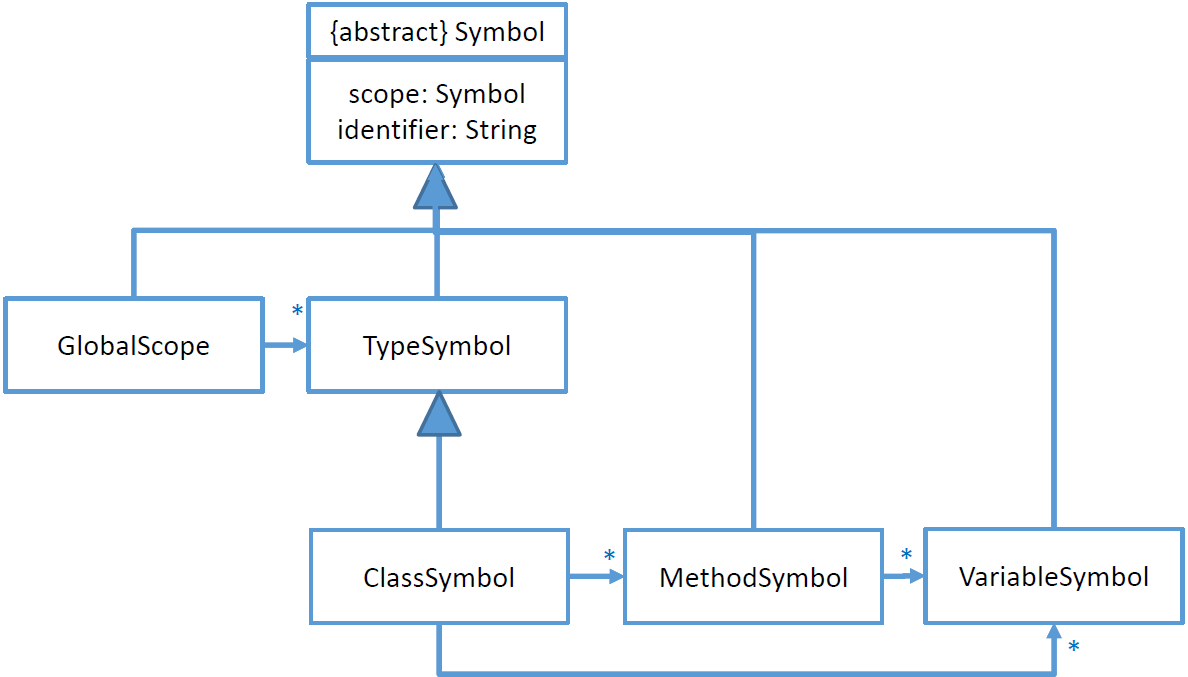
\includegraphics[width=0.7\linewidth]{symboltabelle_design.png}
\subsubsection{Detailiertere Beziehungen}
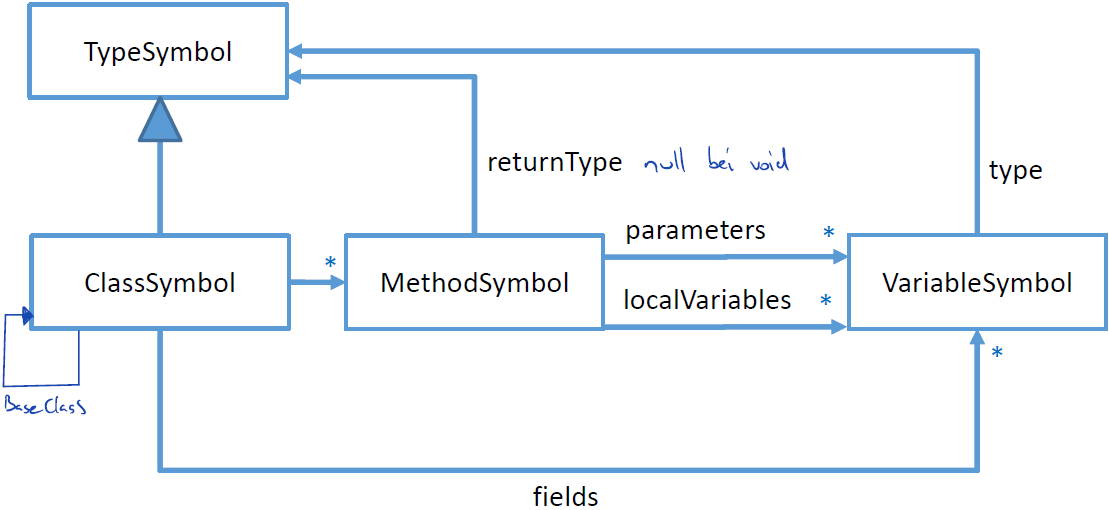
\includegraphics[width=0.7\linewidth]{symboltabelle_design_detailliert.png}
\subsubsection{Design Aspekte}
\textbf{Typinfo für Variable-Symbol}
\begin{itemize}
    \item Zuerst unaufgelöst (Identifier)
\end{itemize}
\textbf{Weitere Infos}
\begin{itemize}
    \item Klassen: Basisklasse
\end{itemize}
\textbf{Lokale Variablen}
\begin{itemize}
    \item Deklarationsbereich merken (Statements)
\end{itemize}
\textbf{Erweitertes Typ-Design}
\begin{itemize}
    \item Klassen
    \item Basistypen (int, boolean, string)
    \item Arrays
\end{itemize}
\textbf{Erweitertes Variablen-Design:}\\ 
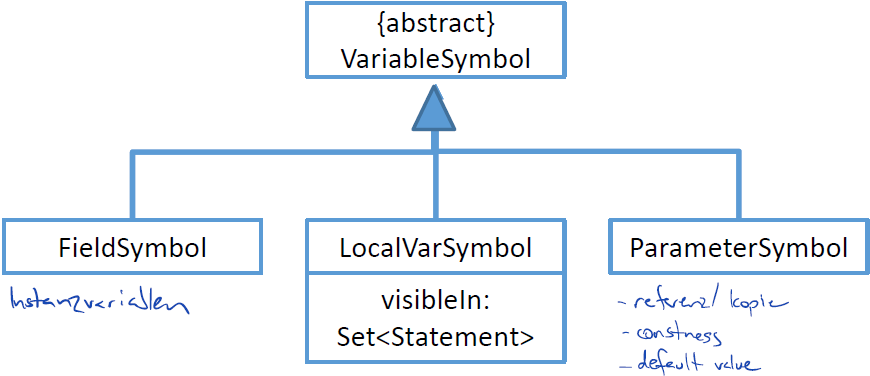
\includegraphics[width=0.5\linewidth]{var_design.png}
\subsubsection{AST Verknüpfung}
\begin{itemize}
    \item Symboltabelle enthält Mapping Symbol $\rightarrow$ AST
    \item Für alle Deklarationen
\end{itemize}
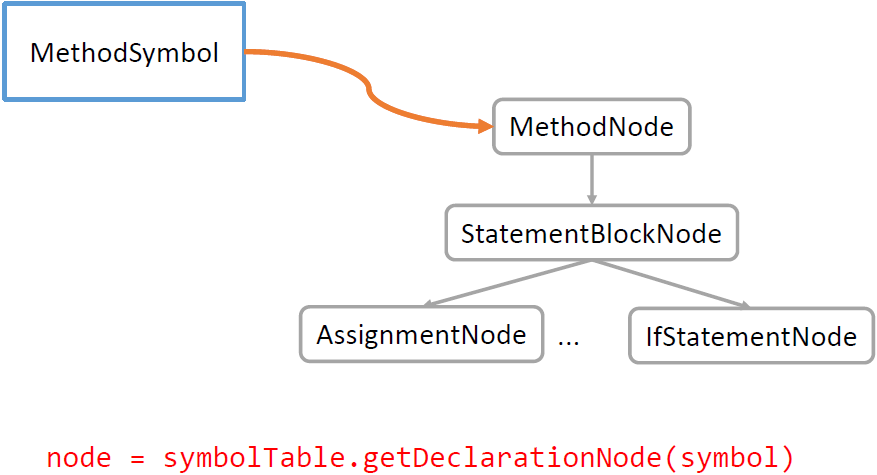
\includegraphics[width=0.6\linewidth]{ast_symboltabelle.png}

\subsection{Global Scope}
\begin{itemize}
    \item Mehrere Klassen im Programm
\end{itemize}

\subsection{Shadowing}
\begin{itemize}
    \item Deklarationen in inneren Bereichen verdecken gleichnamige von äusseren Bereichen
    \item Hiding: Bei gleicher Member-Name bei Vererbung
\end{itemize}

\subsection{Vorgehen}
\begin{enumerate}
    \item Konstruktion der Symboltabelle
    \item Typen in Tabelle auflösen 
    \item Deklaration in AST auflösen 
    \item Typen in AST auflösen
\end{enumerate}

\subsubsection{1. Konstruktion der Symboltabelle}
\textbf{AST traversieren}
\begin{itemize}
    \item Beginne mit Global Scope
    \item Pro Klasse, Methode, Parameter, Variable: Symbol in übergeordnetem Scope einfügen
    \item Explizit und/oder mit Visitor
\end{itemize}
\textbf{Forward-Referenzen $\rightarrow$ Typ-Namen und Designatoren noch nicht auflösen!}
\begin{itemize}
    \item Da vlt noch nicht alle Klassen in der Symboltabelle sind
\end{itemize}

\subsubsection{2. Typen in Tabelle auflösen}
\begin{itemize}
    \item Für Variablentype, Parametertyp, Rückgabetyp etc.
    \item Brauche Suche für Identifier auf Symboltabelle
    \begin{itemize}
        \item Starte mit innerstem Scope
        \item Suche stetig nach aussen ausbreiten
        \item Zuletzt in Global Scope suchen, ansonsten nicht vorhanden
    \end{itemize}
\end{itemize}
\begin{lstlisting}
Symbol find(Symbol scope, String identifier) {
    if(scope == null) {
        return null; // nicht im global scope
    }
    for (Symbol declaration : scope.allDeclarations()) {
        if(declaration.getIdentifier().equals(identifier)) {
            return declaration;
        }
    }
    return find(scope.getScope(), identifier); // rekursiv in nächst höheren Bereich
}
\end{lstlisting}

\subsubsection{3. Deklaration in AST auflösen}
\begin{itemize}
    \item Traversiere Ausführungscode in AST
    \item Jeden Designator auflösen, Deklaration zuordnen
\end{itemize}
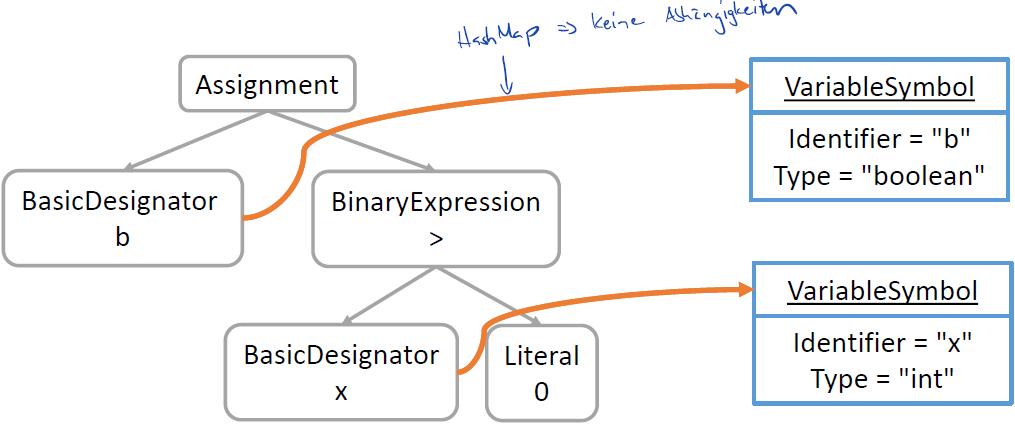
\includegraphics[width=0.7\linewidth]{dekl_in_ast.png}

\subsubsection{4. Typen in AST bestimmen}
\textbf{Typ zu jeder Expression zuordnen}
\begin{itemize}
    \item Literal: definierter Typ
    \item Designator: Typ der Deklaration
    \item Unary/BinaryExpression: Resultat des Operators
\end{itemize}
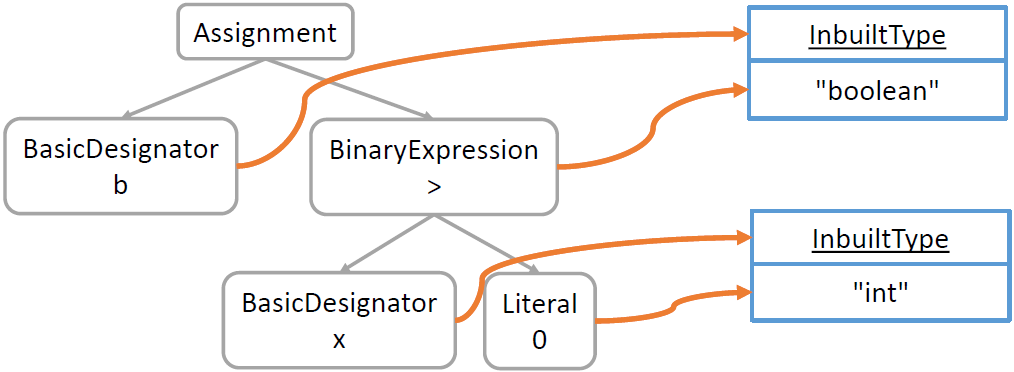
\includegraphics[width=0.7\linewidth]{typen_in_ast.png}\\
\textbf{Ablauf der Typenbestimmung:}
\begin{itemize}
    \item Post-Order-Traversierung
    \item AST am besten nicht erweitern sondern Maps in Symboltabelle verwenden
\end{itemize}
\subsubsection{Typauflösung per Visitor}
\begin{lstlisting}
@Override
public void visit(BinaryExpressionNode node) {
    Visitor.super.visit(node); // post-order travers
    var leftType = symboltable.findType(node.getLeft());
    var rightType = symboltable.findType(node.getRight());
    // ... 
    switch(node.getOperator()) {
        case PLUS -> {
            checkType(leftType, globalScope.getIntType());
            checkType(rightType, globalScope.getIntType());
            symboltable.fixType(node, globalScope.getIntType());
        }
        // ...
    }
}
\end{lstlisting}

\subsection{Semantic Checks}
\begin{itemize}
    \item Alle Designatoren beziehen sich auf Variablen/Methoden
    \item Typen stimmen bei Operatoren
    \item Kompatible Typen bei Zuweisungen
    \item Argumentliste passt auf Parameterliste
    \item Bedingungen in if, while sind boolean
    \item Return Ausdruck passt
    \item Keine Mehrfachdeklaration
    \item Kein Identifier ist reservierts Keyword
    \item Exakt eine main() Methode
    \item Array length  is read-only
    \item Kein Exit ohne Return (ausser void)
    \item Lesen von unitialisierten Variablen
    \item Null-Dereferenzierung
    \item Ungültiger Array-Index
    \item Division by Zero
    \item Out of Memory bei new()
\end{itemize}
        \newpage
        \section{Code Generator}
\subsection{Aufgabe}
\textbf{Erzeugung von ausführbarem Maschinencode}
\begin{itemize}
    \item Input: Zwischendarstellung (Symboltabelle + AST)
    \item Output: Maschinencode
\end{itemize}
\textbf{Mögliche Zielmaschinen}
\begin{itemize}
    \item Reale Maschine, z.B. intel 64, ARM Prozessor
    \item VM, z.B. JVM, .NET CLI
\end{itemize}

\subsection{Unsere Zielmaschine}
\textbf{Kernkonzepte}
\begin{itemize}
    \item Virtueller Stack-Prozessor: keine Register
    \item Branch Instructions (Goto): Programmfluss steuern
    \item Metadaten
\end{itemize}

\subsection{Stack Prozessor}
\begin{itemize}
    \item Instruktionen benutzen Auswertungs-Stack
    \item Keine Register wie auf echten Prozessoren
\end{itemize}

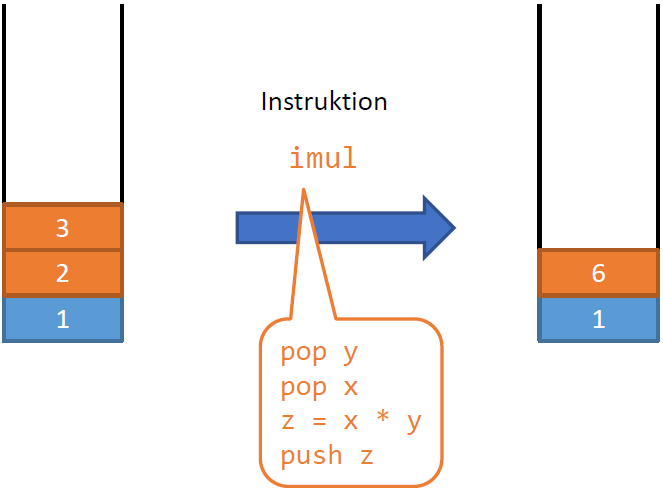
\includegraphics[width=0.5\linewidth]{stack_prozessor.png}

\subsection{Auswertungs-Stack}
\begin{itemize}
    \item Jede Instruktion hat definierte Anzahl von Pop- und Push-Aufrufen
    \item Eigener Stack pro Methodenaufruf
    \item Stack hat unbeschränkte Kapazität
\end{itemize}
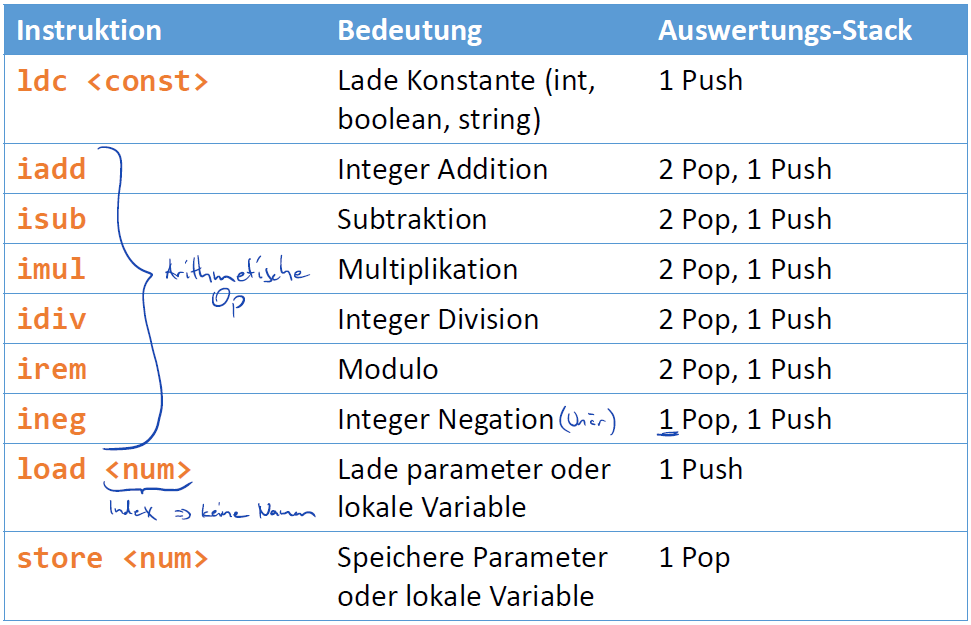
\includegraphics[width=0.5\linewidth]{instruktionen.png}

\subsubsection{Load/Store Nummerierungen}
\begin{itemize}
    \item \textit{this} Referenz: Index 0
    \item Danach, $n$ \textbf{Parameters}: Index $1..n$
    \item Danach, $m$ \textbf{lokale Variablen}: Index $n+1...n+m$
\end{itemize}
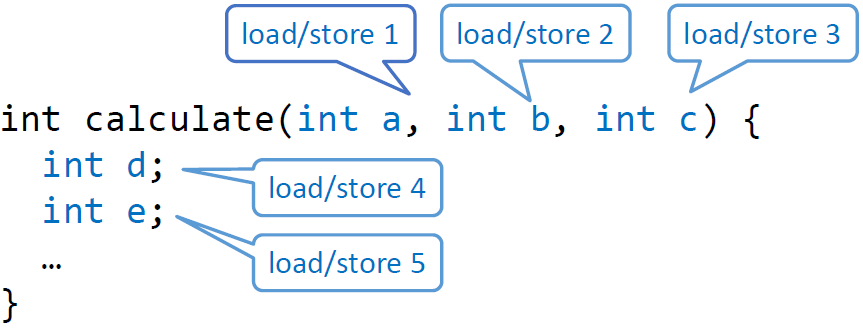
\includegraphics[width=0.5\linewidth]{load_store.png}

\subsubsection{Compare-Instruktionen}
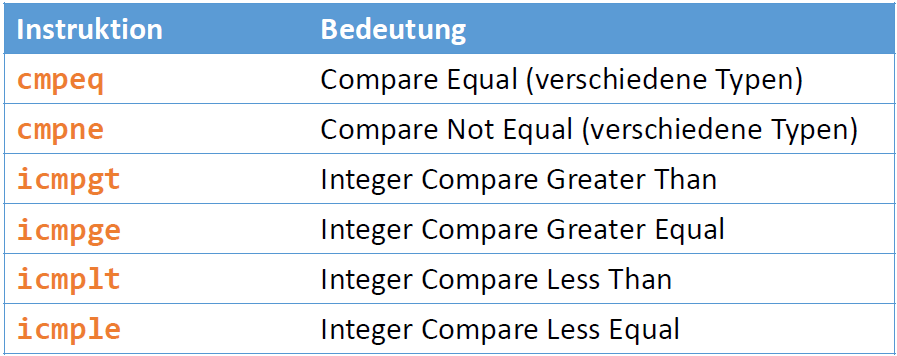
\includegraphics[width=0.5\linewidth]{compre_instruktionen.png}\\
\textbf{Pop right, Pop left, Push boolean}

\subsubsection{Branch-Instruktionen}
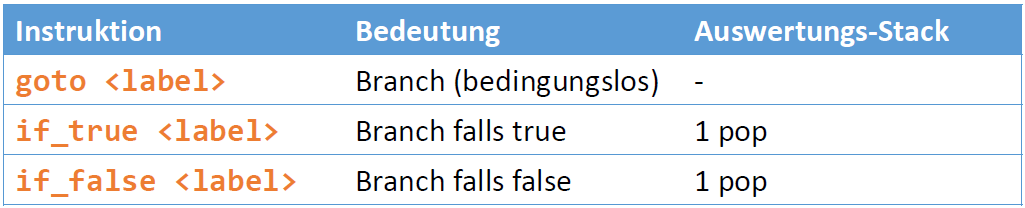
\includegraphics[width=0.5\linewidth]{branch_instruktionen.png}\\

\subsubsection{Metadaten}
\begin{itemize}
    \item Zwischensprache kennt alle Informationen zu
    \begin{itemize}
        \item Klassen (Namen, Typen der Fields und Methoden)
        \item Methoden (Namen, Parametertypen und Rückgabetyp)
        \item Lokale Variablen (Typen)
    \end{itemize}
    \item Kein direktes Speicherlayout festgelegt
    \item Nicht enthalten
    \begin{itemize}
        \item Namen von lokalen Variablen und Parameter
        \item Diese sind nur nummeriert
    \end{itemize}
\end{itemize}
\textbf{Verwendung:}
\begin{itemize}
    \item Speicherplatz-Allozierung
    \item Fehlermeldungen
    \item Funktionsaufrufe
\end{itemize}

\subsection{Code Generierung}
\begin{enumerate}
    \item Traversiere Symboltabelle: Erzeuge Bytecode Metadaten
    \item Traversiere AST pro Methode (Visitor): Erzeuge Instruktionen via Bytecode Assembler
    \item Serialisiere in Output Format
\end{enumerate}

\subsubsection{Backpatching}
\begin{itemize}
    \item Branch Offsets auflösen
    \item Label: relativer Instruktions-Offset ab Ende der aktuellen Branch-Instruktion
\end{itemize}

\subsubsection{Template-Basierte Generierung}
\begin{itemize}
    \item Postorder-Traversierung: Kinder zuerst besuchen
    \item Jeweils Template für erkanntes Teilbaum-Muster anwenden
\end{itemize}

\subsubsection{Short-Circuit Semantik}
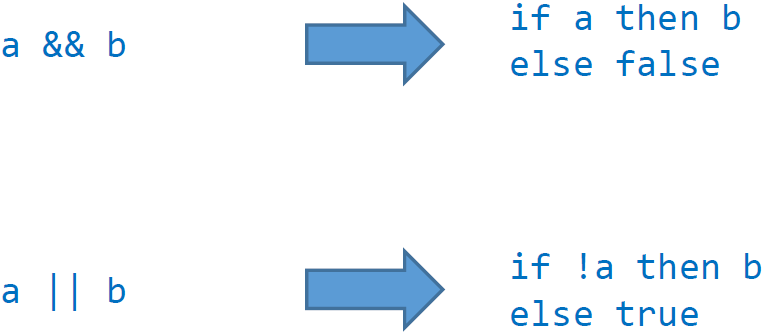
\includegraphics[width=0.5\linewidth]{short_circuit.png}

\subsubsection{Methodenaufruf}
\textbf{Statisch}
\begin{itemize}
    \item Vordefinierte Methoden: $readInt()$ etc.
\end{itemize}
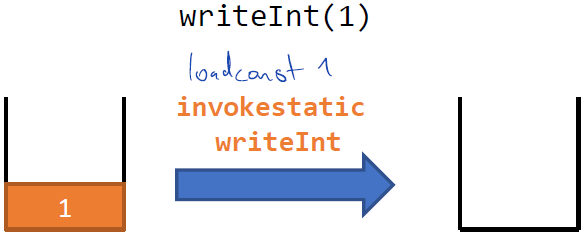
\includegraphics[width=0.4\linewidth]{static1.png}
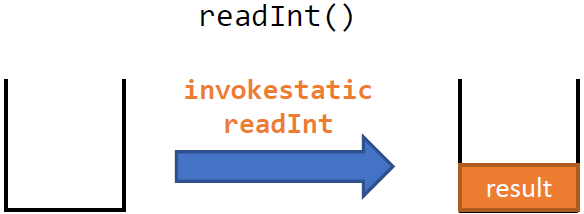
\includegraphics[width=0.4\linewidth]{static2.png}
\vspace{1cm}\\

\textbf{Virtuell}
\begin{itemize}
    \item Alle anderen Methoden
\end{itemize}
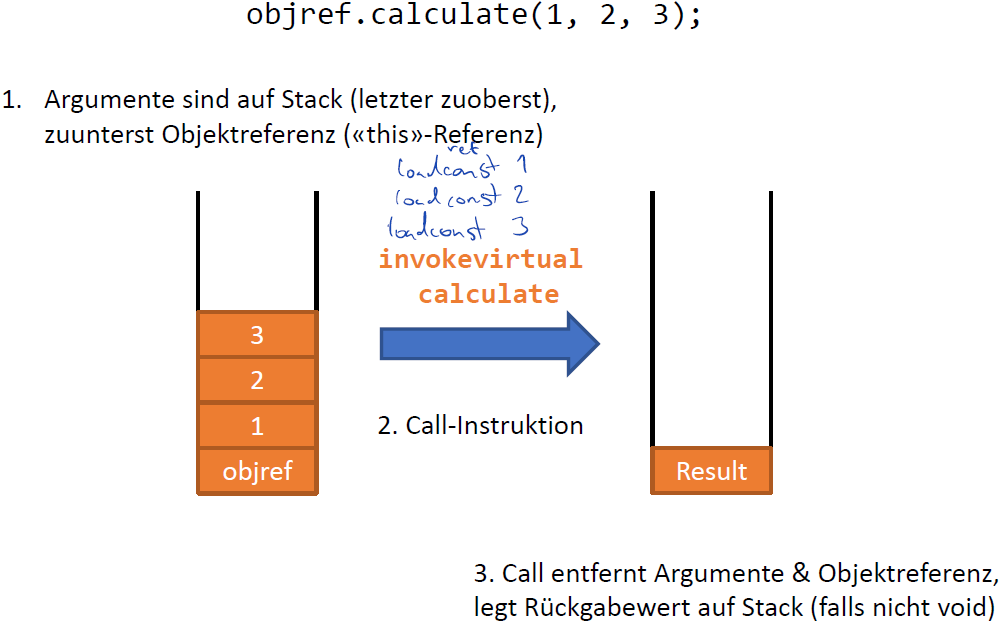
\includegraphics[width=0.5\linewidth]{virt.png}

\subsubsection{Parameter \& Rückgabe}
\begin{lstlisting}
int sum(int x, int y) {
    return x + y;
}

load 1 // load param x
load 2 // load param y
iadd // x + y
ret // return from method (auch bei void, max 1 Wert auf Stack)
\end{lstlisting}
        \newpage
        \section{Virtual Machine}
Hypotetische Maschine mit virtuellem Prozessor
\begin{itemize}
    \item Eigener Instruktionssatz: Intermediate Language
    \item Hülle um den realen Prozessor
\end{itemize}
\textbf{Nutzen:}
\begin{itemize}
    \item Mehrplattformen
    \item Mehrsprachigkeit
    \item Sicherheit
\end{itemize}

\subsection{Loader}
\begin{itemize}
    \item Lädt Zwischencode (File) in Speicher
    \item Alloziert Speicher (Metadaten für Klassen, Methoden, Variablen, Code)
    \item Definiert Layouts (Speicherbereiche für Fields/Variablen/Parameter)
    \item Address Relocation
    \begin{itemize}
        \item Löst Verweise auf zu Methoden, Typen, andere Assemblies
    \end{itemize}
    \item Initiiert Programmausführung
    \item Optional: Verifier
\end{itemize}

\subsubsection{Verifier}
\textbf{Erkenne und verhindere falscher IL-Code}
\begin{itemize}
    \item Statische Analyse zur Ladezeit
    \item Fehler in Compuler, böswillige Manipulationen
\end{itemize}
\textbf{Denkbare Fehler}
\begin{itemize}
    \item Typfehler
    \item Stack-Überlauf oder Unterlauf
    \item Nicht definierte Variablen/Methoden/Klassen
    \item Illegale Sprünge
\end{itemize}
\textbf{Alternative: Überprüfung zur Laufzeit}

\subsubsection{Metadaten}
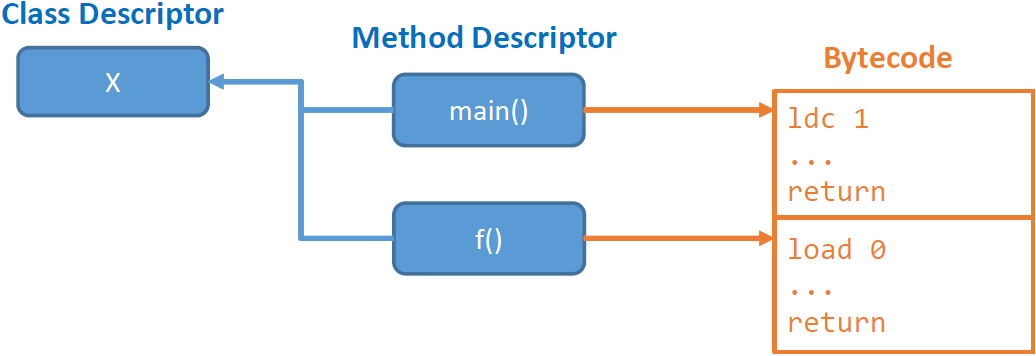
\includegraphics[width=0.5\linewidth]{metadaten.png}

\subsubsection{Deskriptoren}
\textbf{Laufzeitinfo für Typen \& Methoden}
\begin{itemize}
    \item Typen: Klassen, Arrays oder Basistypen
    \item Klassen: Field-Typen
    \item Methoden: Typen von Parameter \& Locals, Rückgabetyp, Bytecode
    \item Zusätzlich bei Klassen: Parent-Klasse, virtual Method Table
\end{itemize}
\vspace{0.5cm}
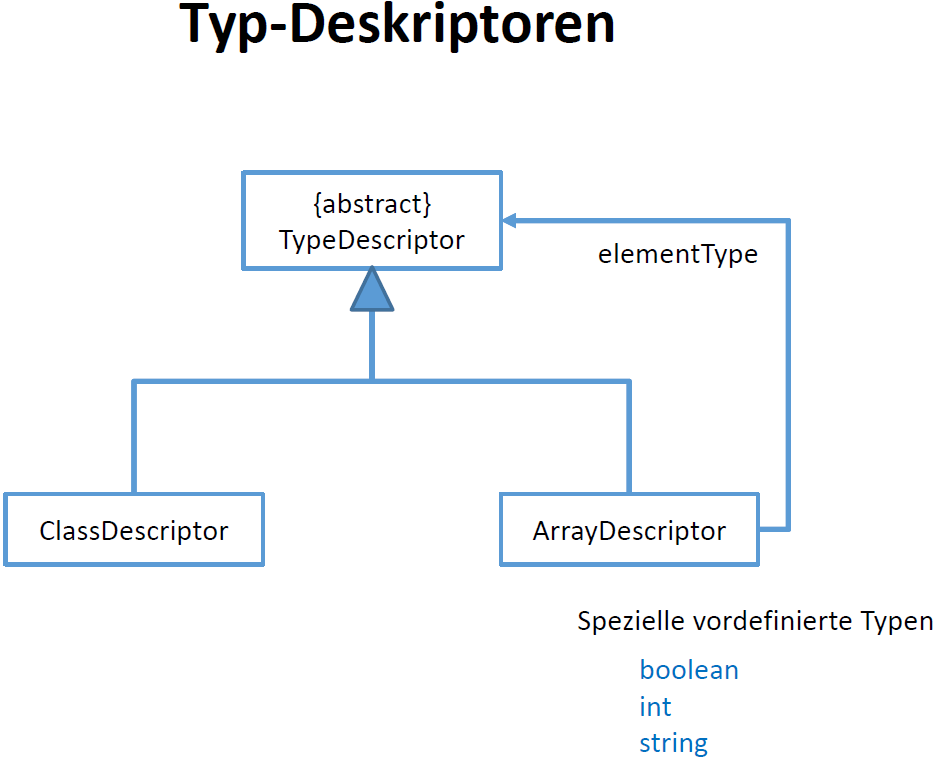
\includegraphics[width=0.5\linewidth]{typ_deskriptoren.png}
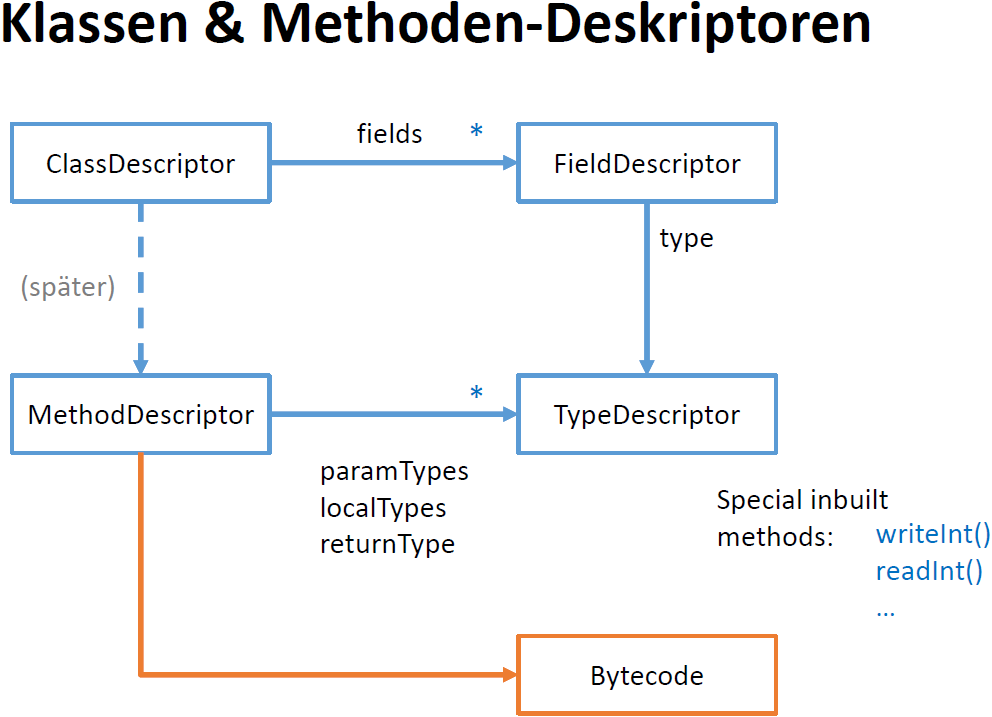
\includegraphics[width=0.5\linewidth]{klassen_deskriptoren.png}

\subsubsection{Bytecode Loading}
\begin{itemize}
    \item Von File direkt in Speicher geladen
    \item \textbf{Patching/Fixup:} Argumente in Instruktion anpassen
    \item Referenzen auf entsprechende Metadaten
\end{itemize}
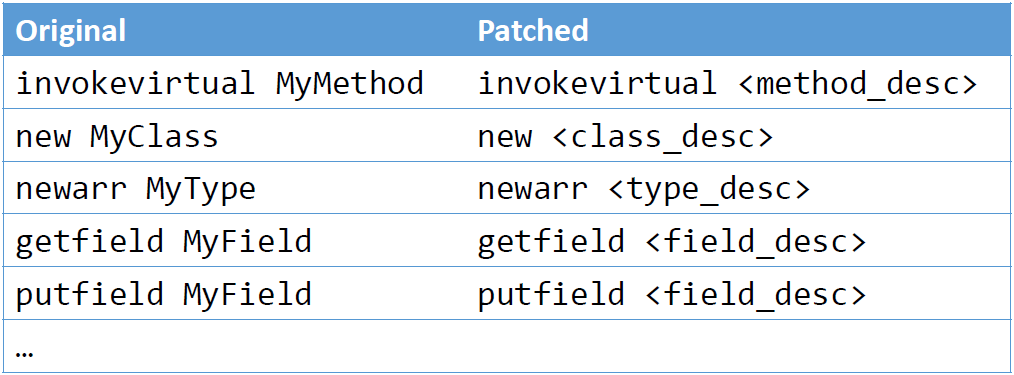
\includegraphics[width=0.5\linewidth]{patching.png}
\subsubsection{Patching}
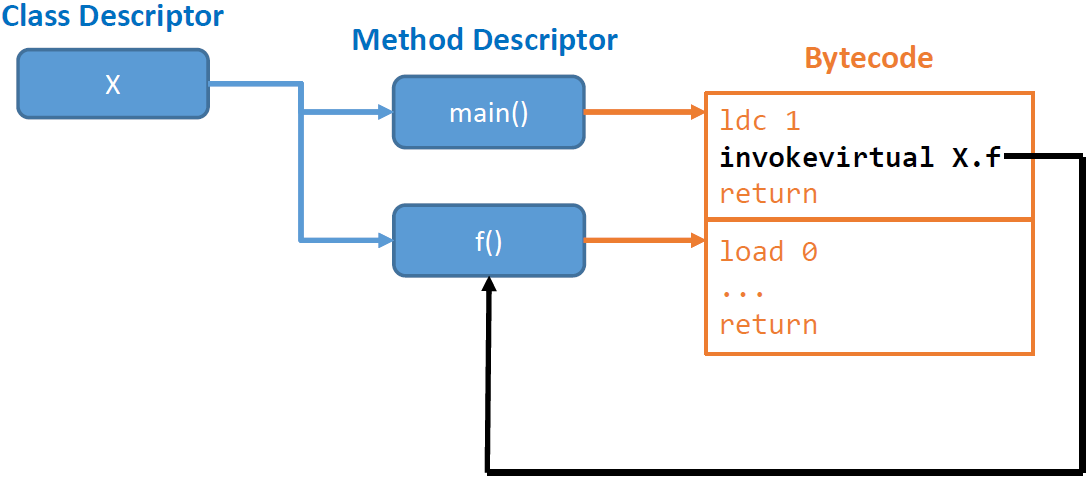
\includegraphics[width=0.5\linewidth]{patching2.png}

\subsubsection{VM: Managed \& Unmanaged}
\textbf{Kleine Unmanaged Teile neben der Java VM}
\begin{itemize}
    \item Heap und HW-Excution (JIT)
\end{itemize}

\includegraphics[width=0.5\linewidth]{managed.png}

\subsection{Interpreter}
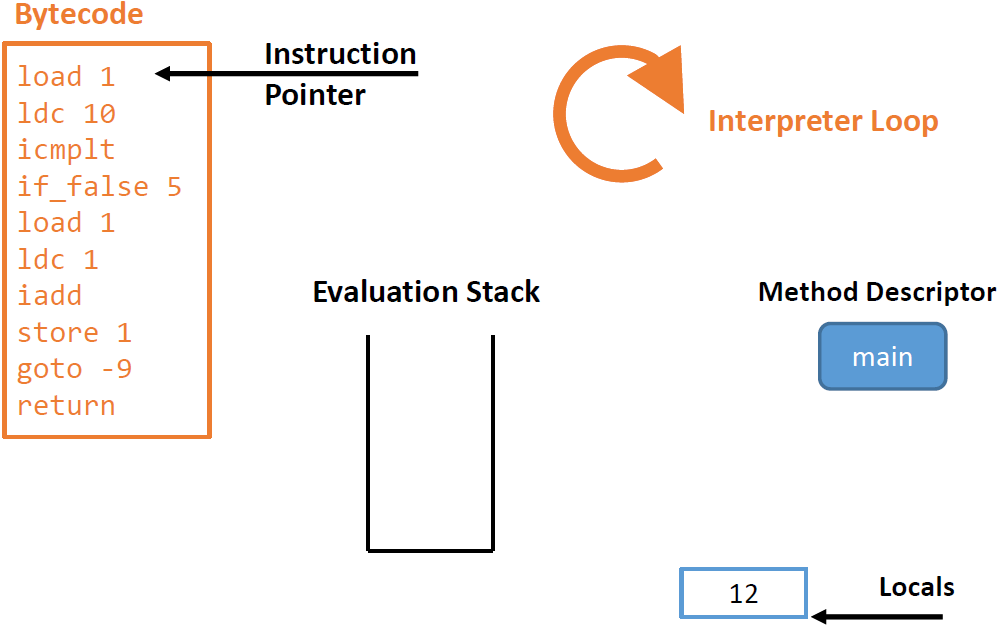
\includegraphics[width=0.7\linewidth]{interpreter.png}
\subsubsection{Bestandteile}
\textbf{Interpreter Loop}
\begin{itemize}
    \item Emuliert Instruktion nach der anderen
\end{itemize}
\textbf{Instruction Pointer (IP)}
\begin{itemize}
    \item Adresse der nächsten Instruktion
\end{itemize}
\textbf{Evaluation Stack}
\begin{itemize}
    \item Für virtuellen Stack Prozessor
\end{itemize}
\textbf{Locals \& Parameter}
\begin{itemize}
    \item Für aktive Methoden
\end{itemize}
\textbf{Method Deskriptor}
\begin{itemize}
    \item Für aktive Methode
\end{itemize}

\subsubsection{Implementation}
\begin{lstlisting}
private void execute(Instruction instruction) {
    var operand = instruction.getOperand();
    var frame = activeFrame();
    switch (instruction.getOpCode()) {
    case LDC -> push(operand);
    case ACONST_NULL -> push(null);
    case IADD -> {
        int right = checkInt(pop());
        int left = checkInt(pop());
        push(left + right);
    }
    // ISUB, IMUL, IDIV, IREM, INEG, BNEG
    case CMPEQ -> {
        var right = pop();
        var left = pop();
        if(left != null) {
            push(left.equals(right));
        } else {
            push(left == right);
        }
    }
    // CMPNE
    case ICMPLT -> {
        int right = checkInt(pop());
        int left = checkInt(pop());
        push(left < right);
    }
    // ICMPLE, ICMPGT, ICMPGE
    case IF_TRUE -> {
        if(checkBoolean(pop())) {
            frame.setInstructionPointer(frame.getInstructionPointer() + checkInt(operand));
        }
    }
    // IF\_FALSE
    case GOTO -> {
        frame.setInstructionPointer(frame.getInstructionPointer() + checkInt(operand));
    }
    case LOAD -> {
        push(getParamOrLocal(checkInt(operand))); 
    }
    case STORE -> {
        setParamOrLocal(checkInt(operand), pop());
    }
    case ALOAD -> {
        var arrayIndex = checkInt(pop());
        var pointer = checkPointer(pop());
        if(pointer == null) {
            throw new InvalidBytecodeException("Null pointer");
        }
        var length = heap.getArrayLength(pointer);
        if(arrayIndex < 0 || arrayIndex >= length) {
            throw new InvalidBytecodeException("Index out of bound");
        }
        var element = heap.readElement(pointer, arrayIndex);
        push(element);
    }
    // ASTORE
    case ARRAYLENGTH -> {
        var pointer = checkPointer(pop());
        if(pointer == null) {
            throw new InvalidBytecodeException("Null pointer");
        }
        push(heap.getArrayLength(pointer));
        
    }
    // GETFIELD
    case PUTFIELD -> {
        var field = checkFieldDescriptor(operand);
        var index = field.getIndex();
        var value = pop();
        checkType(value, field.getType());
        var instance = checkPointer(pop());
        if(instance == null) {
            throw new InvalidBytecodeException("Accessing uninitialized object");
        }
        heap.writeField(instance, index, value);
    }
    case NEW -> {
        var type = checkClassDescriptor(operand);
        var instance = newObject(type);
        push(instance);
    }
    case NEWARRAY -> {
        var length = checkInt(pop());
        if(length < 0) {
            throw new InvalidBytecodeException("Negative array size");
        }
        var descriptor = checkArrayDescriptor(operand);
        var pointer = heap.allocateArray(descriptor, length);
        for (int i = 0; i < length; i++) {
            heap.writeElement(pointer, i, defaultValue(descriptor.getElementType()));
        }
        push(pointer);
    }
    case INSTANCEOF -> instanceofTest(operand);
    case CHECKCAST -> checkCast(operand);
    case INVOKESTATIC -> invokeStatic(operand);
    case INVOKEVIRTUAL -> invokeVirtual(operand);
    case RETURN -> returnCall();
    default -> throw new InvalidBytecodeException("Unsupported instruction opcode");
    }
}
\end{lstlisting}

\subsubsection{Prozedurale Unterstützung}
\textbf{Methodenaufrufe}
\begin{itemize}
    \item invokevirtual: Aufruf neuer Methode
    \item return: Rücksprung aus Methode
\end{itemize}
\textbf{Activation Frame}
\begin{itemize}
    \item Datenraum einer Methode
    \item Parameter, lokale Variablen, temporäre Auswertungen
\end{itemize}
\textbf{Call Stack}
\begin{itemize}
    \item Stack der Activation Frames gemäss Aufrufreihenfolge
    \item Design:
    \begin{itemize}
        \item Managed im Interpreter: OO Darstellung für Komfort
        \item Unmanaged bei HW Execution: Kontinuierlicher Speicherblock für Effizienz
    \end{itemize}
\end{itemize}
\subsubsection{Gesamtbild}
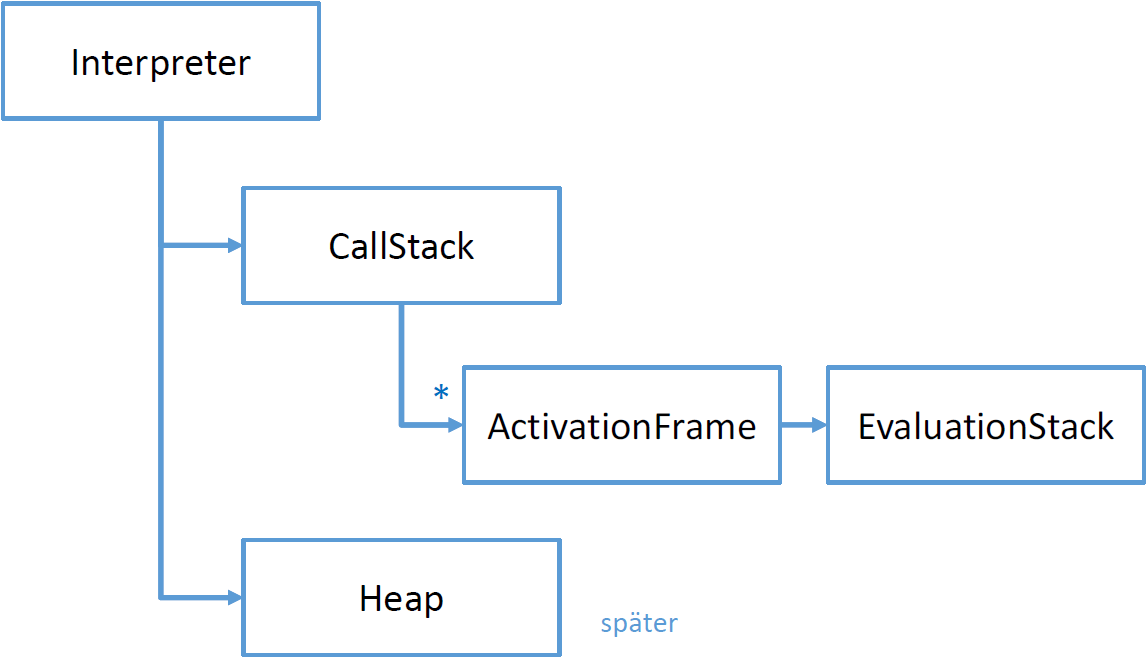
\includegraphics[width=0.5\linewidth]{gesamtbild.png}

\subsubsection{Verifikation im Interpreter}
\textbf{Korrekte Benutzung der Instruktionen}
\begin{itemize}
    \item Typen stimmen (e.g. \textit{checkInt()})
    \item Methodenaufrufe stimmen (Argumente, Rückgabe etc.)
    \item Sprünge sind gültig
    \item Op-Codes stimmen 
\end{itemize}

\subsubsection{Sicherheitsmassnahmen}
\begin{itemize}
    \item Korrekter Bytecode und Typkonsistenz prüfen
    \item Variablen immer initialisieren (auch lokale)
    \item Checks durchführen (Null, Array-Index etc.)
    \item Stack Overflow und Underflow Detection
\end{itemize}

\subsubsection{Interpretation vs. Kompilation}
\textbf{Interpreter ist ineffizient}
\begin{itemize}
    \item Dafür flexibel und einfach zu entwickeln
    \item Akzeptabel für selten ausgeführten Code
\end{itemize}
\textbf{Kompilierter HW-Prozessor Code ist schneller}
\begin{itemize}
    \item Just-In-Time (JIT) Compilation für Hot Spots
    \item Kompilation kostet, Laufzeit macht es (allenfalls) wett 
\end{itemize}
        \newpage
        \section{Object-Orientierung}
\subsection{Objekte zur Laufzeit}
\begin{itemize}
    \item Ablage erzeugter Objekte auf Heap
    \item Heap: Linearer Adressraum
\end{itemize}
\textbf{Wiso werden Objekte nicht auf dem Stack augelegt?}
\begin{itemize}
    \item Sie würden Methoden-Ende nicht überleben, sondern mit Activation Frame zerstört werden.
\end{itemize}
\textbf{Objekt Lebenszeit}
\begin{itemize}
    \item Nicht an Methodeninkarnatiion gebunden
\end{itemize}

\subsubsection{Deallokation}
\begin{itemize}
    \item Keine Hierarchie unter Objekten
    \item Keine hierarchische Lebensdauer
    \item Deallokation verursacht Lücken
\end{itemize}

\subsection{Unmanaged Memory in Java}
\begin{itemize}
    \item Speicher über Java Native Access allozieren
    \item Raw Heap kann keine Java Referenzen speichern! Stattdessen Map verwenden (\textit{HashMap\textless Long, Object\textgreater})
\end{itemize}
\begin{lstlisting}
import com.sun.jna.Memory;

Memory heap = new Memory(HEAP_SIZE);

long value = heap.getLong(address); // 64-bit lesen, address = offset im Heap
// ... 
heap.setLong(address, value);
\end{lstlisting}

\subsubsection{Objektblock im Raw Heap}
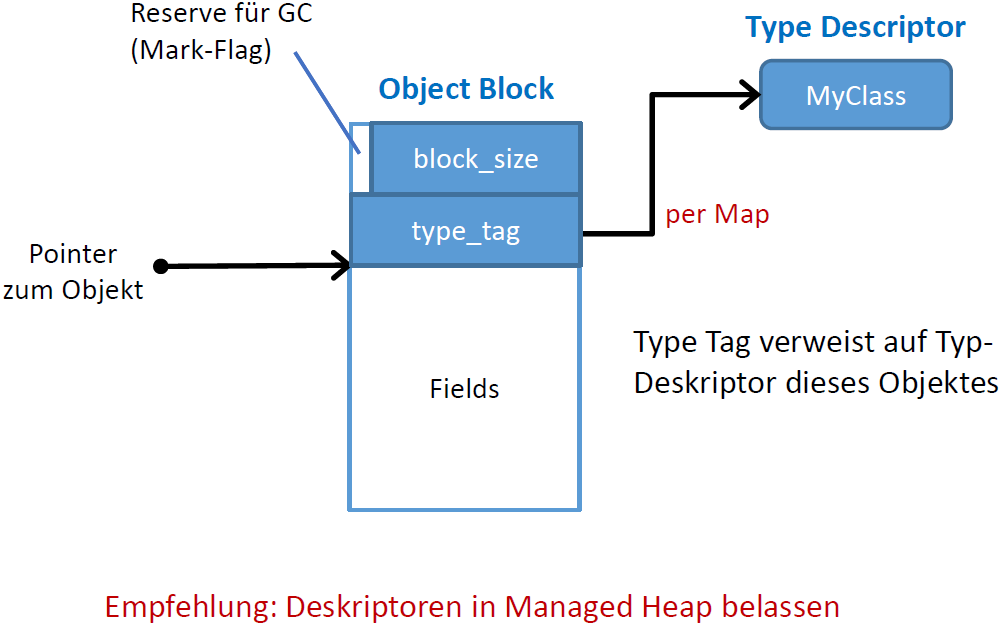
\includegraphics[width=0.5\linewidth]{raw_heap.png}
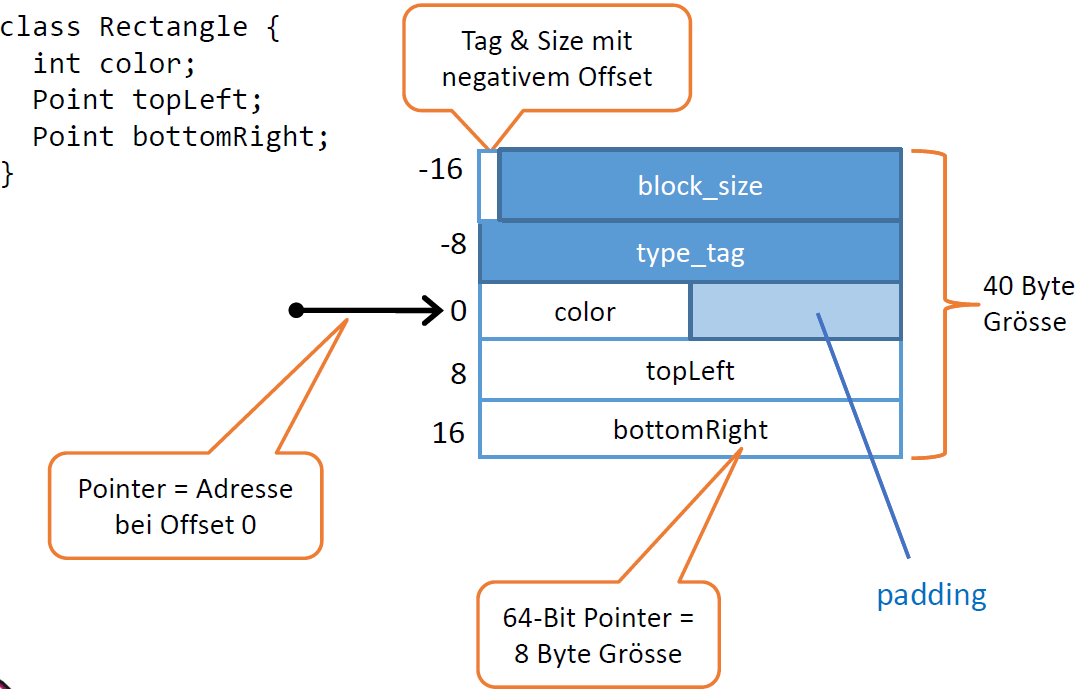
\includegraphics[width=0.5\linewidth]{raw_heap2.png}

\subsubsection{Array Block}
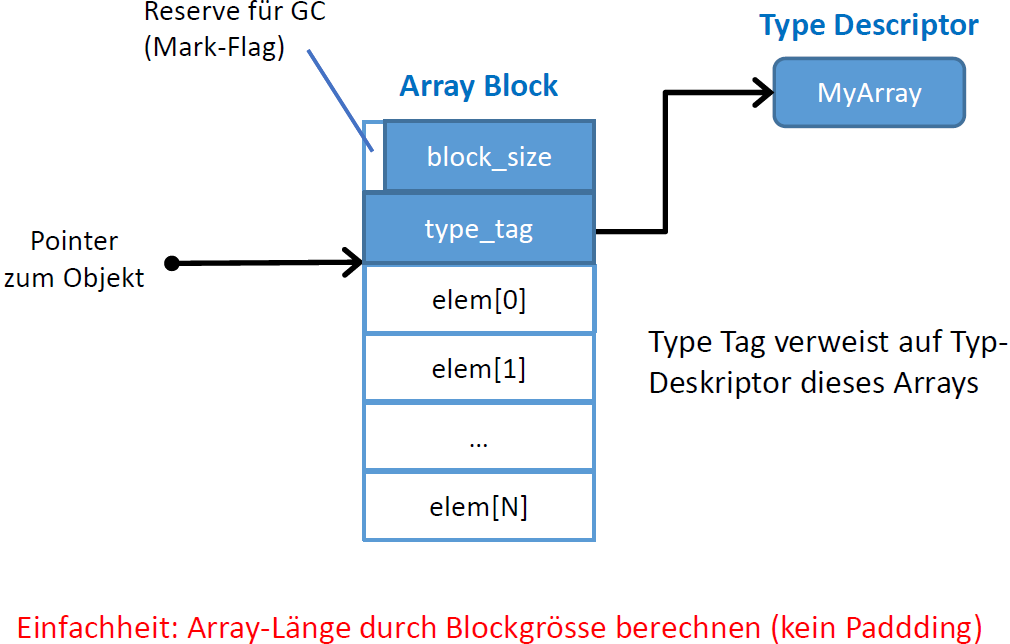
\includegraphics[width=0.5\linewidth]{array_block.png}

\subsubsection{Heap-Allokation}
\begin{lstlisting}
Pointer allocate(int size, TypeDescriptor type) {
    int blockSize = size + 16; // Mit Header
    if(freePointer + blockSize > limit) {
        throw new VMException("Out of Memory");
    }
    long address = freePointer;
    freePointer += blockSize;
    heap.setLong(address, blockSize);
    setTypeDescriptor(type, address);
    address += 16;
    return new Pointer(address);
}

Pointer allocateObject(ClassDescriptor type) {
    int size = type.getAllFields().length * 8; // Einfaches Layout 
    return allocate(size, type);
}

Pointer allocateArraay(ArrayDescriptor type, int length) {
    int size = length * 8;
    return allocate(size, type);
}
\end{lstlisting}
        \newpage
        \section{Typ Polymorphismus}
\textbf{Dynamische Typ-Bestimmung}
\begin{itemize}
    \item Typ-Deskriptor = Dynamischer Typ des Objektes
\end{itemize}
\subsection{Ancestor Tables}
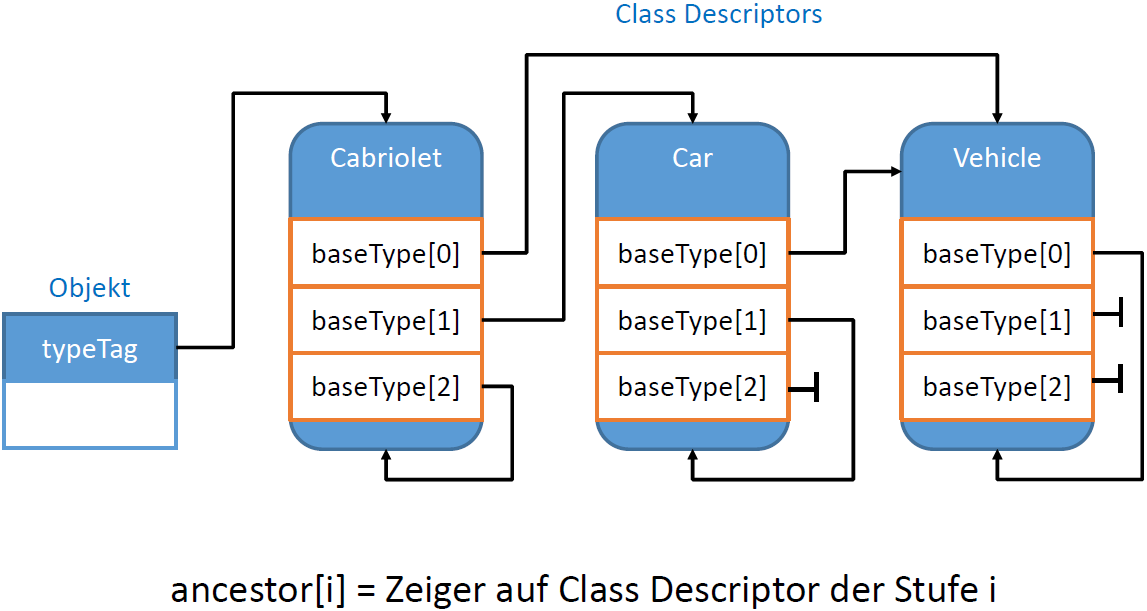
\includegraphics[width=0.6\linewidth]{ancestor_tables.png}
\subsection{Implementierung}
\begin{lstlisting}
private void instanceofTest(Object operand) {
    var instance = checkPointer(pop());
    if (instance == null) {
        push(false);
    } else {
        var targetType = checkClassDescriptor(operand);
        push(typeTest(instance, targetType));
    }
}

private void checkCast(Object operand) {
    var instance = checkPointer(pop());
    push(instance);
    var targetType = checkClassDescriptor(operand);
    if (!typeTest(instance, targetType)) {
        throw new VMException("Invalid cast");
    }
}
\end{lstlisting}

\subsection{Virtual Method Table}
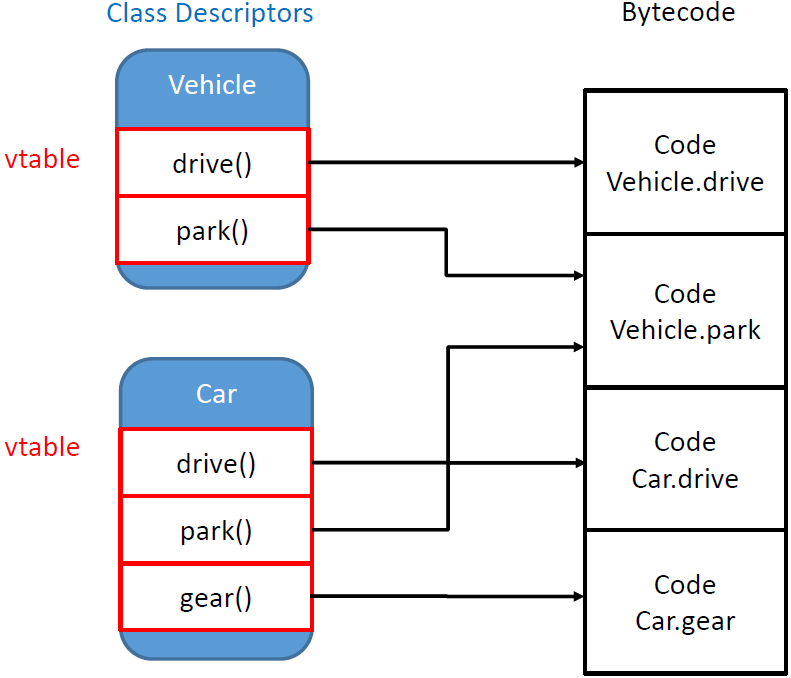
\includegraphics[width=0.4\linewidth]{virtual_method_table.png}
\subsubsection{Lineare Erweiterung}
\textbf{Jede virtuelle Methode hat einen Eintrag}
\begin{itemize}
    \item Methoden der Basisklasse oben
    \item Neu deklarierte Methoden der Subklasse unten
    \item Funktioniert nur bei Single Inheritance
\end{itemize}
\subsubsection{Method Position}
\begin{itemize}
    \item Jede virtuelle Methode hat fixe Position in vtable
    \item Position ist statisch bekannt im deklarierten Typ
\end{itemize}
\subsubsection{Method Descriptor}
\begin{itemize}
    \item Zusätzliche Indirektion über Methoden-Deskriptor
    \item Interpreter braucht Infos zu Typen von Params/Locals
\end{itemize}
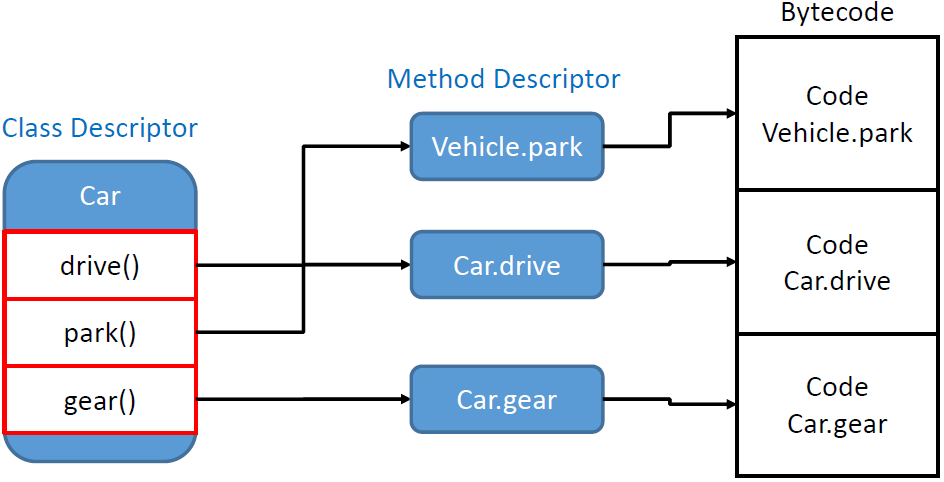
\includegraphics[width=0.5\linewidth]{method_descriptor.png}
\subsubsection{Implementation}
\begin{lstlisting}
private void invokeVirtual(Object operand) {
    var staticMethod = checkMethodDescriptor(operand);
    var parameterTypes = staticMethod.getParameterTypes();
    var arguments = new Object[parameterTypes.length];
    for (int index = arguments.length - 1; index >= 0; index--) {
        arguments[index] = pop();
        checkType(arguments[index], parameterTypes[index]);
    }
    var target = checkPointer(pop());
    invokeVirtual(staticMethod, target, arguments);
}

private void invokeVirtual(MethodDescriptor staticMethod, Pointer target, Object[] arguments) {
    if (target == null) {
        throw new VMException("Null dereferenced");
    }
    var type = checkClassDescriptor(heap.getDescriptor(target));
    var position = staticMethod.getPosition();
    var vtable = type.getVirtualTable();
    var dynamicMethod = vtable[position];
    var locals = initLocals(dynamicMethod.getLocalTypes());
    if (useJIT && jitEngine.supports(dynamicMethod)) {
        performJITCall(dynamicMethod, arguments);
    } else {
        callStack.push(new ActivationFrame(dynamicMethod, target, arguments, locals));
    }
}
\end{lstlisting}

\subsection{Interface Support}
\begin{itemize}
    \item Interfaces global durchnummerieren
    \item Pro Class Descriptor eine Interface Tabelle (itable)
    \begin{itemize}
        \item Interfaces nach Nummer = Position eintragen
    \end{itemize}
    \item Einträge in \textit{itable} verweisen auf \textit{vtable}
    \item Class Deskriptor verweist auf \textit{itable} (ibase-Pointer)
\end{itemize}
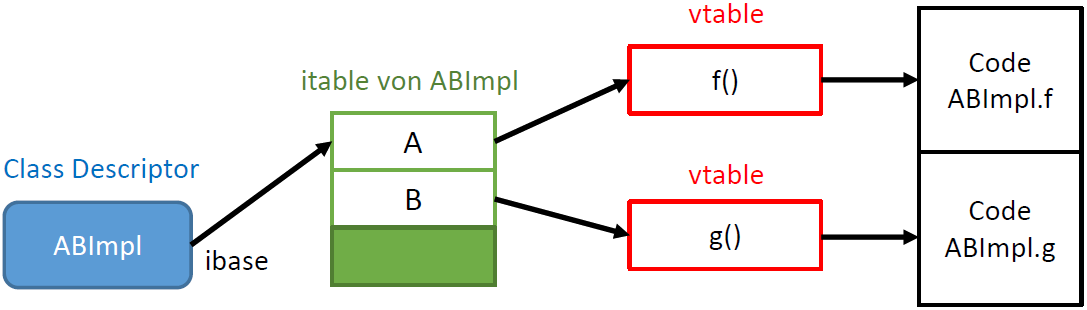
\includegraphics[width=0.6\linewidth]{interface_support.png}

\subsubsection{Verzahnte Interface Tabelle}
\textbf{Grund}
\begin{itemize}
    \item Einfache Interface Tabellen sind ein Speicherproblem
    \item Lange itables bei vielen Interfaces
    \item Viele Lücken wegen globaler Nummeriereung
\end{itemize}
\textbf{Konzept}
\begin{itemize}
    \item \textit{itables} im Speicher kollisionsfrei übereinanderlegen
    \item Muss nun prüfen, ob Eintrag für Typ gültig ist (Vermerk des Class Descriptors in \textit{vtable})
\end{itemize}
\subsubsection{Verschiedene Offsets}
\begin{itemize}
    \item Verzahnung auch mit veschiedenen Offsets möglich
\end{itemize}

\subsubsection{Gesamtbild}
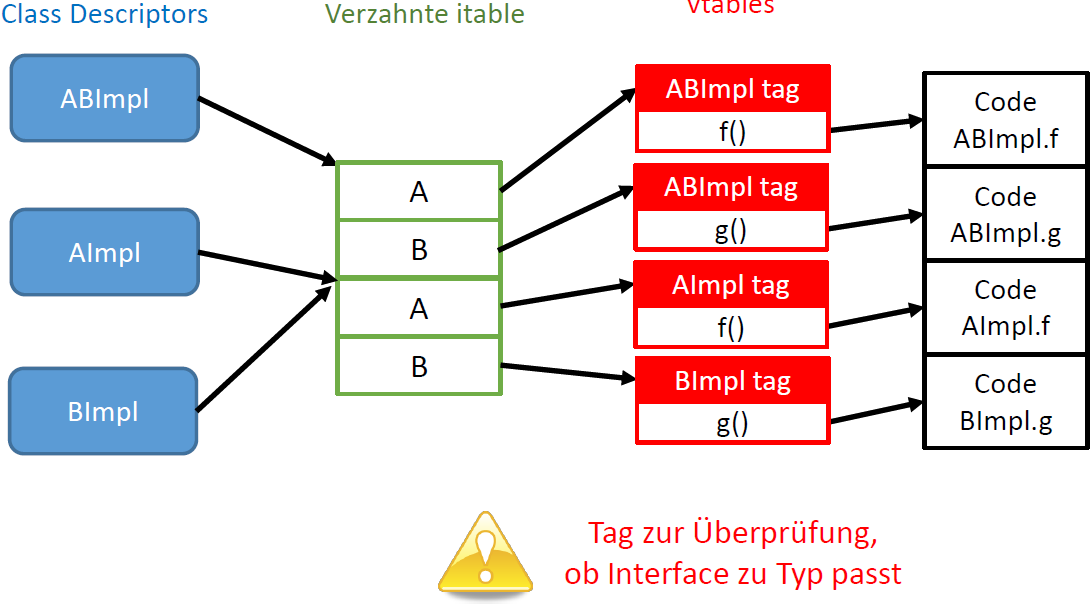
\includegraphics[width=0.6\linewidth]{gesamtbild_interface_support.png}

        \newpage
        \section{Garbage Collection}
\textbf{Typ-Deskriptor Zweck}
\begin{itemize}
    \item Ancestor Table für Typ-Test \& Cast
    \item Virtual Method Table für Dynamic Dispatch
    \item Interpreter Metadata bei Field- / Array Typen
    \item \textbf{Neu:} Pointer Offsets für Garbage Collection
\end{itemize}

\subsection{Explizite Freigabe}
\begin{itemize}
    \item Delete Statement zum Deallozieren eines Objektes
\end{itemize}
\subsubsection{Probleme}
\begin{itemize}
    \item Dangling Pointers: Referenz auf gelöschtes Objekt
    \item Memory Leaks: Verweiste Objekte, die nicht abräumbar sind
\end{itemize}

\subsubsection{Dangling Pointer}
\begin{itemize}
    \item Zeigt auf Lücke oder falsches Objekt im Heap
    \item Lese nicht berechtigten Speicher (Security Issue)
    \item Überschreibe fremden Speicher (Safety + Security Issue)
\end{itemize}

\subsubsection{Memory Leak}
\begin{itemize}
    \item Unbenötigtes Objekt, das nicht löschbar ist
    \item Es gibt keine benutzbaren Referenzen mehr darauf
\end{itemize}

\subsection{Garbage Collection}
\begin{itemize}
    \item Laufzeitsystem kümmert sich um die automatische Freigabe von Garbage
    \item Garbage = Objekte, die nicht mehr erreichbar sind und daher nicht mehr gebraucht werden
\end{itemize}
\textbf{Ziel:}
\begin{itemize}
    \item Memory Safety
    \item Keine Dangling Pointers
    \item Keine Memory Leaks
\end{itemize}

\subsubsection{Reference Counting}
\begin{itemize}
    \item RC pro Objekt
    \item Anzahl eingehender Referenzen
    \item Zyklische Objektstrukturen werden mit Reference Counting nie zu Garbage
\end{itemize}
\textbf{Vorteil}
\begin{itemize}
    \item Sofortige Deallokation
\end{itemize}
\textbf{Nachteile}
\begin{itemize}
    \item Falsch bei Zyklen
    \item Ineffizient
\end{itemize}
\textbf{\textcolor{red}{Untauglich}}

\subsubsection{Transitive Erreichbarkeit}
\begin{itemize}
    \item Objekte beibehalten, die das Programm noch zugreifen könnte
    \item Ausgehend von Ankerpunkten (Root Set)
\end{itemize}
\textbf{Root Set}
\begin{itemize}
    \item Referenzen in statischen Variablen
    \item Referenzen in Activation Frames auf Call Stack
    \item Referenzen in Register
\end{itemize}

\subsection{Mark \& Sweep Algorithmus}
\textbf{Mark Phase}
\begin{itemize}
    \item Markiere alle erreichbaren Objekte
\end{itemize}
\textbf{Sweep Phase}
\begin{itemize}
    \item Lösche alle nicht markierten Objekte
\end{itemize}
\subsubsection{Mark Phase}
\begin{lstlisting}
private void mark() {
    for(var root: getRootSet(stack)) {
        traverse(root);
    }
}

private void traverse(Pointer current) {
    if(current == null) {
        return;
    }
    long block = heap.getAddress(current) - Heap.BLOCK_HEADER_SIZE;
    if(!isMarked(block)) {
        setMark(block);
        for(var next: getPointers(current)) {
            traverse(next);
        }
    }
}
\end{lstlisting}

\subsubsection{Rekursive Traversierung}
\begin{itemize}
    \item GC braucht zusätzlich Speicher für Stack
    \item Problematisch, da Speicher bei GC meist sowiso knapp ist
    \item Es exisitieren Algorithmen zur Traversierung ohne Zusatzspeicher (Pointer Rotation Algo)
\end{itemize}

\subsubsection{Sweep Phase}
\begin{itemize}
    \item Linearer Scan über den gesamten Heap, alle Blöcke
\end{itemize}
\begin{lstlisting}
private void sweep() {
    var current = Heap.HEAP_START;
    while(current < Heap.HEAP_SIZE) {
        if(!isMarked(current) && !freeList.contains(current)) {
            free(current);
        }
        clearMark(current);
        current += heap.getBlockSize(current);
    }
}

private void free(long address) {
    freeList.add(address);
}
\end{lstlisting}

\subsection{Ausführungszeitpunkt}
\textbf{Delayed Garbage Collection}
\begin{itemize}
    \item Garbage wird nicht sofort erkannt und freigegeben
    \item GC läuft spätestens, wenn der Heap voll ist (Check beim Allozieren)
    \item Eventuell prophylaktisch früher
\end{itemize}

\subsection{Stop \& Go}
\begin{itemize}
    \item GC läuft sequentiell und exklusiv
    \item Mutator = Produktives Programm
    \item Mutator ist während GC unterbrochen
\end{itemize}
\includegraphics[width=0.6\linewidth]{stop_go.png}

\subsection{Root Set Erkennung}
\textbf{Pointer auf dem Call Stack}
\begin{itemize}
    \item Pointers in Parameter
    \item Pointers in lokalen Variablen
    \item Pointers auf Evaluation Stack
    \item this-Referenz
\end{itemize}

\subsection{Pointers im Objekt}
\begin{lstlisting}
private Iterable<Pointer> getPointers(Pointer current) {
    var list = new ArrayList<Pointer>();
    var descriptor = heap.getDescriptor(current);
    if(descriptor instanceof ClassDescriptor classDescriptor) {
        var fields = classDescriptor.getAllFields();
        for(var i = 0; i < fields.length; i++) {
            var type = fields[i].getType();
            if(isPointerType(type)) {
                var value = heap.readField(current, i);
                if(value != null) {
                    list.add((Pointer) value);
                }
            } 
        }
    } else if (descriptor instanceof ArrayDescriptor arrayDescriptor) {
        var length = heap.getArrayLength(current);
        for (int i = 0; i < length; i++) {
            var value = heap.readElement(current, i);
            var type = arrayDescriptor.getElementType();
            if (value != null && isPointerType(type)) {
                list.add((Pointer)value);
            }
        }
    }
    return list;
}

private boolean isPointerType(Object pointer) {
    return pointer instanceof ClassDescriptor || pointer instanceof ArrayDescriptor;
}
\end{lstlisting}

\subsection{Free List}
\begin{itemize}
    \item Freie Blöcke linear verketten
\end{itemize}
\subsubsection{Neue Heap Allozierung}
\begin{itemize}
    \item Traversiere Free List bis zu passendem Block
    \item Überschuss des Blockes wieder in free List einreihen
\end{itemize}
\includegraphics[width=0.6\linewidth]{free_list.png}
\subsubsection{Heap Block Layout}
\includegraphics[width=0.6\linewidth]{heap_block_layout.png}
\subsubsection{Strategien}
\textbf{First Fit}
\begin{itemize}
    \item Keine Sortierung
    \item Suche erst passenden Block
\end{itemize}
\textbf{Best Fit}
\begin{itemize}
    \item Nach aufsteigender Grösse sortiert
    \item Unbrauchbar kleine Fragmente
\end{itemize}
\textbf{Worst Fit}
\begin{itemize}
    \item Nach absteigender Grösse sortiert
    \item Finde passenden Block sofort
\end{itemize}
\textbf{Segregated Free List}
\begin{itemize}
    \item Mehrere Free Lists mit verschiedenen Grössenklassen
    \item e.g. 64..128, 128..196, 196..259, ...
\end{itemize}
\textbf{Benachbarte freie Blöcke verschmelzen}
\begin{itemize}
    \item Am einfachsten in der Sweep Phase
\end{itemize}
\textbf{Buddy System}
\begin{itemize}
    \item Diskrete Blockgrössen nach Adresse geordnet
    \item Exponentielle Blockgrösse
    \item Sehr schnelles Verschmelzen \& Allozieren \& Freigabe
    \item Aber grosse interne Fragmentierung (unbrauchbare Reste)
\end{itemize}

\section{GC Vertiefung}
\textbf{Pointers in C++}
\begin{itemize}
    \item expliziter Zahlenwert
    \item Jedes Wort kann Pointer sein
    \item Keine GC Metadaten in C/C++
\end{itemize}

\subsection{Finalizer}
\begin{itemize}
    \item Methode, die vor Löschen des Objektes läuft (Abschlussarbeit wie z.B. Verbindung schliessen)
    \item Von GC initiiert, wenn Objekt Garbage geworden ist
\end{itemize}
\begin{lstlisting}
class Block {
    @Override 
    protected void finalize() {
        // ...
    }
}
\end{lstlisting}
\subsubsection{Separate Finalisierung}
\begin{itemize}
    \item Finalizer wird nicht in GC-Phase ausgeführt, sondern erst später
\end{itemize}
\textbf{Gründe}
\begin{itemize}
    \item Finalizer dauert evtl. beliebig lange (blockiert sonst GC)
    \item Finalizer kann neue Objekte allozieren (korrumpiert GC)
    \item Programmierfehler im Finalizer (evtl. Crash des GC)
    \item Finalizer kann Objekt wieder weiterleben lassen (Resurrection)
\end{itemize}

\subsubsection{Resurrection}
\begin{itemize}
    \item Finalizer kann bewirken, dass Objekt wieder lebendig wird und kein Garbage mehr ist
    \item Nicht nur das eigene Objekt, sondern auch indirekt andere Objekte können wiederauferstehen
\end{itemize}
\includegraphics[width=0.6\linewidth]{resurrection.png}

\subsubsection{Internals}
\textbf{Finalizer Set}
\begin{itemize}
    \item Registrierte Finalizer
\end{itemize}
\textbf{Pending Queue}
\begin{itemize}
    \item Noch auszuführende Finalizer
    \item Garbage mit Finalizer werden in Pending Queue eingetragen
    \item Einfügen bewirkt Resurrection: Neue GC Phase nötig
\end{itemize}

\subsubsection{Konsequenzen}
\textbf{GC braucht 2 Mark Phasen}
\begin{itemize}
    \item Markiere und erkenne Garbage mit Finalizer
    \item Markiere von Pending Queue erneut, dann Sweep
\end{itemize}
\textbf{Objekt mit Finalizer braucht min 2 GC Durchläufe bis zur Freigabe}
\begin{itemize}
    \item Speicher kann evtl. nicht schnell genug frei werden
\end{itemize}

\subsubsection{Programmieraspekte}
\begin{itemize}
    \item Reihenfolge der Finalizer ist unbestimmt
    \item Laufen beliebig verzögert
    \item Sind nebenläufig zum Hauptprogramm
\end{itemize}

\subsection{Weak Reference}
\begin{itemize}
    \item Zählt nicht als Referenz für GC
    \item Für Objekt Caches
\end{itemize}
\textbf{Internals}
\begin{itemize}
    \item Indirektion via Weak Reference Table
    \item GC Mark ignoriert Table-Einträge
    \item GC Sweep nullt Einträge, falls Zielobjekte gelöscht
\end{itemize}

\subsection{Externe Fragmentierung}
\textbf{Viele kleine Lücken im Heap durch Allozieren \& Free}
\begin{itemize}
    \item Spätere grössere Allokation passt in keine Lücke
    \item Obschon Summe der freien Blöcken genügend wäre
\end{itemize}
\includegraphics[width=0.6\linewidth]{externe_frag.png}

\subsection{Compacting GC}
\begin{itemize}
    \item Auch Mark \& Copy GC
    \item Allokation am Heap-Ende (supereffizient)
    \item GC schiebt Objekte wieder zusammen
    \item Bei Verschieben müssen Referenzen nachgetragen werden
    \item Konservative Methode daher unmöglich (C/C++ nicht möglich)
\end{itemize}
\includegraphics[width=0.5\linewidth]{compacting_gc.png}

\subsection{Inkrementeller GC}
\begin{itemize}
    \item GC soll quasi-parallel zum Mutator laufen
    \item Nur kleinste Unterbrüche (Inkrements)
    \item Kein Stop \& Go / Stop the World
\end{itemize}
\includegraphics[width=0.6\linewidth]{inkr_gc.png}
\subsubsection{Generational GC}
\textbf{Zeitspiegelungsheuristik}
\begin{itemize}
    \item Junge Objekte: kurze Lebensdauer
    \item Alte Objekte: lange Lebensdauer
\end{itemize}
\includegraphics[width=0.5\linewidth]{generational_gc.png}\\
\textbf{Root Sets bei Generationen}
\begin{itemize}
    \item Referenzen von alten zu neuen Generationen: Zusätzlicher Root Set der neuen Gen
    \item Write Barriers: Schreiben von Referenzen in alte Generationen erkennen
    \item Bei GC der alten Generationen müssen auch neuere mit aufgeräumt werden
\end{itemize}

\subsubsection{Partitioned GC}
\begin{itemize}
    \item Heap in Partitionen zerlegen
    \item Ziel: kurze GC Pausen
    \item Nebenläufiges Markieren mit Snapshots: Relevante nebenläufige Updates erkennen
    \item GC fokussiert auf Partitionen mit viel Garbage
    \item Evakuiere lebende Objekte in neue Partitionen
\end{itemize}
\textbf{Problem}
\begin{itemize}
    \item Zyklischer Garbage zwischen Partitionen
    \item Braucht immer noch Full GC (Stop the World)
\end{itemize}
\includegraphics[width=0.3\linewidth]{partitioned_gc1.png} $\rightarrow$
\includegraphics[width=0.3\linewidth]{partitioned_gc2.png} $\rightarrow$
\includegraphics[width=0.3\linewidth]{partitioned_gc3.png}

\subsection{Wellenausbreitungsmodell}
\includegraphics[width=0.6\linewidth]{wellenausbreitungsmodell.png}

\subsection{Isolationsproblem}
\begin{itemize}
    \item Referenzzuweisung durch Mutator während GC
    \item Kritisch: Neue Referenz von dunkelblau zu weiss
    \item \textbf{Heilung:} Quelle oder Ziel hellblau färben (Write Barrier)
\end{itemize}
\includegraphics[width=0.6\linewidth]{isolationsproblem.png}

        \newpage
        \section{Just-In-Time Compiler}
\begin{itemize}
    \item Effizientere Ausführung als Interpretation
    \item Bytecode direkt in nativen Prozessor-Code übersetzen und ausführen
    \item Nicht unbedingt alles, sondern nur kritische Teile
\end{itemize}

\subsection{Hot Spot}
\begin{itemize}
    \item Performance-kritisher Code Abschnitt
    \item Wird häufig ausgeführt
    \item JIT-Kompilierung loht sich hierfür am meisten
\end{itemize}

\subsection{Profiling}
\begin{itemize}
    \item Interpreter zählt Ausführung gewisser Code-Teile (Methoden, Traces (Code-Pfade))
    \item Falls häufig ausgeführt, JIT für den Teil anwerfen
\end{itemize}

\subsection{Vorgehen}
\includegraphics[width=0.4\linewidth]{jit_vorgehen.png}

\subsection{Intel 64 Architektur}
\textbf{Spezielle Register}
\begin{itemize}
    \item RSP: Stack Pointer
    \item RBP: Base Pointer
    \item RIP: Instruction Pointer
\end{itemize}
\includegraphics[width=0.5\linewidth]{intel1.png}
\includegraphics[width=0.5\linewidth]{intel2.png}

\subsubsection{Elementare Instruktionen}
\includegraphics[width=0.5\linewidth]{elementare_instruktionen.png}
\includegraphics[width=0.5\linewidth]{arithm_instruktionen.png}

\subsubsection{IDIV Vorbereiten}
\begin{itemize}
    \item Fixe 128-bit Division von RDX:RAX
    \item Setze RDX je nach RAX
    \begin{itemize}
        \item 0 falls RAX $>=$ 0
        \item -1 falls RAX $<$ 0
    \end{itemize}
\end{itemize}
\includegraphics[width=0.5\linewidth]{cdq.png}

\subsection{Register Allokation}
\textbf{Lokale Register Allokation}
\begin{itemize}
    \item Für Ausdrucksauswertung (Evaluation Stack)
    \item Evaluation Stack Einträge auf Register abbilden
    \item Cross Compiler führt Stack an belegten Register 
    \item Pro übersetzte Bytecode-Instruktion wird Stack nachgeführt
\end{itemize}
\textbf{Globale Register-Allokation}
\begin{itemize}
    \item Veriablen in Register speichern
    \item Deutlich schneller als Speicherzugriffe
    \item Parameter werden oft als Register übergeben (Calling Convention)
\end{itemize}
\textbf{Registeranzahl ist beschränkt!}

\subsection{Register Clobbering}
\begin{itemize}
    \item Evakuiere in neues Register bei Instruktionen mit fixem Operand (z.B. IDIV)
\end{itemize}
\subsubsection{Register Relocation}
\begin{itemize}
    \item Umkopieren in anderes Register
\end{itemize}
\includegraphics[width=0.5\linewidth]{register_relocation.png}

\subsection{Intel Branches}
\begin{itemize}
    \item Bedingte Sprünge basierend auf Condition Code
    \item Condition Code aus vorherigem Vergleich
\end{itemize}
\includegraphics[width=0.5\linewidth]{branch_instruktionen_intel.png}

        \newpage
        \section{Code Optimierung}
\subsection{Aufgabe}
\begin{itemize}
    \item Transformation von Intermediate Representation / Maschinencode zu effizienteren Version 
    \item Mögliche Intermediate Representations
    \begin{itemize}
        \item AST + Symbol Table
        \item Bytecode
        \item andere (z.b. Three Address Code)
    \end{itemize}
    \item Meist Serie von Optimierungsschritten
\end{itemize}

\subsection{Optimierte Arithmetik}
\textbf{Multiplikation, Division und Modulo mit Zweierpotenz}\\ 
\[ x * 32 = x << 5\] 
\[ x / 32 = x >> 5\] 
\[ x \% 32 = x \& 31\] 

\subsection{Algebraische Vereinfachung}
\textbf{mittels Template-Based Code Generierung}\\
\includegraphics[width=0.5\linewidth]{alebra_vereinfachung.png}
\includegraphics[width=0.5\linewidth]{alebra_vereinfachung2.png}

\subsection{Loop-Invariant Code}
\textbf{Invarianter Code aus der Schlaufe herausschieben}
\begin{lstlisting}
while (x < N * M) {
    k = y * M;
    x = x + k;
}
// Optimiert
k = y * M;
temp = N * M;
while (x < temp) {
    x = x + k;
}
\end{lstlisting}
\subsection{Common Subexpression Elimination}
\textbf{Wiederholt ausgewertete Teilausdrücke}
\includegraphics[width=0.5\linewidth]{subexpr_elimination.png}

\subsection{Dead Code}
\begin{lstlisting}
a = readInt();
b = a + 1;
writeInt(a);
c = b / 2; // Kein Lesen von c: Dead Code
\end{lstlisting}
\subsubsection{Elimination}
\includegraphics[width=0.5\linewidth]{dead_code.png}

\subsection{Redundatnes Lesen und Schreiben (Copy Propagation)}
\includegraphics[width=0.5\linewidth]{copy_propagation.png}

\subsection{Constant Propagation (Constant Folding)}
\includegraphics[width=0.3\linewidth]{constant_propagation.png}\\
\textbf{Danach kann Dead Code oder Duplikate entfernt werden}

\subsection{Partial Redundancy}
\textbf{Beim if-Pfad wird x + 4 zweimal evaluiert}\\
\includegraphics[width=0.5\linewidth]{partial_redundancy.png}

\subsection{Erkennung von Optimierungspotential}
\subsubsection{Static single Assignment}
Code-Transformation für einfachere Analyse \& Optimierung
\begin{itemize}
    \item Jede Variable wird nur einmal im Code zugewiesen
\end{itemize}
\includegraphics[width=0.4\linewidth]{ssa.png}\\ 
\textbf{Komplexer bei Verzweigungen}
\begin{itemize}
    \item Version von Variable nicht immer klar
    \item Phi Function: $\phi (x_1, x_2)$
    \begin{itemize}
        \item $x_1$ bei Pfad1
        \item $x_2$ bei Pfad2
    \end{itemize}
    \item Common Subexpressions werden mit SSA direkt entscheidbar
\end{itemize}
\textbf{SSA Berechnung}
\begin{itemize}
    \item Relativ kompliziert und teuer (besonders Phi)
    \item Günstigere Techniken gewünscht
\end{itemize}

 \subsubsection{Peephole Optimization}
 \begin{itemize}
     \item Optimierung für sehr kleine Anzahl Instruktionen
     \item In JIT-Compiler für Intermediate Code oder Maschinencode benutzt
     \item \textbf{Wende Optimierungsmuster auf Sliding Window an (z.B. 3 Operationen)}
 \end{itemize}
\includegraphics[width=0.5\linewidth]{peephole.png}

\subsubsection{Dataflow Analysis}
\begin{itemize}
    \item Mächtige generische Code-Analyse-Technik
    \item Für viele Optimierungen nützlich
\end{itemize}

\subsection{Summary}
\includegraphics[width=0.5\linewidth]{summary.png}

        \newpage
        \section{Code Analyse}
\subsection{Datenfluss Analyse}
\begin{itemize}
    \item Mächtige und generische Code-Analyse-Technik
    \item Für viele Optimierungen nützlich
\end{itemize}
\subsubsection{Analysebeispiele}
\begin{itemize}
    \item Wo werden uninitialisierte Variablen gelesen?
    \item Ist der Wert einer Variable konstant?
    \item \textbf{Alle Pfade analysieren}
\end{itemize}
\subsubsection{Ansatz}
\textbf{Control Flow Graph erstellen}
\begin{itemize}
    \item Zeigt alle Programm-Pfade
\end{itemize}
\textbf{Datenfluss-Analyse durchführen}
\begin{itemize}
    \item Propagiere Information durch den Graph, bis es stabil ist
\end{itemize}

\subsection{Control Flow Graph}
\begin{itemize}
    \item Repräsentiert alle möglichen Programmpfade (Typischerweise innerhalb einer Methode)
    \item Knoten = Basic Block
    \begin{itemize}
        \item Unterbrochener Code-Abschnitt
        \item Einstieg nur am Anfang: Kein Label in der Mitte
        \item Ausstieg nur am Schluss: Kein Branch in der Mitte
    \end{itemize}
    \item Kante
    \begin{itemize}
        \item Bedingter oder unbedingter Branch
    \end{itemize}
\end{itemize}

\subsubsection{Basic Blocks}
\begin{itemize}
    \item Grenzen durch Branch Entries/Exits gegeben
\end{itemize}
\includegraphics[width=0.2\linewidth]{basic_blocks.png}

\subsubsection{Verknüpfung}
\begin{itemize}
    \item Basic Blocks nach möglichen Branches verknüpfen
\end{itemize}
\includegraphics[width=0.2\linewidth]{cfg.png}

\subsubsection{If-Statement}
\includegraphics[width=0.5\linewidth]{cfg_if.png}

\subsubsection{While-Statement}
\includegraphics[width=0.4\linewidth]{cfg_while.png}

\subsection{Datenflussanalyse}
\begin{itemize}
    \item Fixpunkt-Iteration über CFG
    \begin{itemize}
        \item Propagiere Analyse-Information über Blöcke
        \item Bis es für jeden Block stabil ist
    \end{itemize}
    \item Generische Methode
    \begin{itemize}
        \item Verschiedene Anwendungsfälle
        \item Wird fallspezifisch konfiguriert
    \end{itemize}
\end{itemize}

\subsubsection{State}
\begin{itemize}
    \item Input State und Output State pro Basic Block
    \item Analyse-Information vor und nach einem Block
\end{itemize}

\subsubsection{Transfer}
\begin{itemize}
    \item Abbildung pro Block: Input State $\rightarrow$ Output State
    \item Definiert, was der Block auf Zustand bewirkt
\end{itemize}

\subsubsection{Beispiel}
\begin{itemize}
    \item State = Menge der uninitialisierten Variablen
    \item Transfer = Füge Deklarationen dazu, entferne zugewiesene Variablen
\end{itemize}
\includegraphics[width=0.4\linewidth]{bsp1.png}
\includegraphics[width=0.4\linewidth]{bsp2.png}

\subsubsection{Join}
\begin{itemize}
    \item Kombiniere Output States der Vorgänger zu Input State eines Nachfolgers
    \item Vereinigungsmenge der Vorgänger
\end{itemize}
\includegraphics[width=0.4\linewidth]{join.png}

\subsubsection{Code}
\includegraphics[width=0.5\linewidth]{datenflussanalyse.png}

\subsubsection{Resultat ableiten}
\begin{itemize}
    \item Stabiler Input oder Output State benutzen
    \item z.B. Compiler-Fehler für uninitialisiertes Lesen
\end{itemize}

\subsection{Diskussion}
\textbf{Konservative Analyse}
\begin{itemize}
    \item Betrachtet alle möglichen syntaktischen Pfade
\end{itemize}
\textbf{Kontextfreie Analyse}
\begin{itemize}
    \item Alle Pfade werden gewählt, egal ob Bedingung erfüllt ist
\end{itemize}
\textbf{Fehlermeldung ist auch konservativ}
\begin{itemize}
    \item Falls mindestens ein Pfad mit Fehler existiert = Error
\end{itemize}
\textbf{Fixpunkt-Iteration muss terminieren}
\begin{itemize}
    \item z.B. Falls Menge monoton mit Joins wächst
\end{itemize}
\includegraphics[width=0.3\linewidth]{diskussion.png}

\subsection{Andere Anwendung}
\textbf{Constant Propagation}
\begin{itemize}
    \item Konstante Werte bei Transfer merken
    \item Join = Intersection
\end{itemize}
\textbf{Rückwärts-Propagierung}
\begin{itemize}
    \item Transfer: Out State $\rightarrow$ In State
    \item z.B. Für Dead Code Analysis
\end{itemize}

    \end{multicols*}
\end{document}

























